\chapter{Data Collection}
\label{chap:data-coll}
            

     We extend the Robots\&Hazards dataset~\cite{mantegazza2022outlier} Corridors scenario to train and test the model we built. The dataset is collected by teleoperating the Robomoster S1 through the corridors of the \acrfull{usi} east campus.
     
     This extended version of the dataset is not yet published.
     \\
     \\
    %  \section{Scenarios}
        The Corridors scenario of the Robots\&Hazards dataset consists of 6 corridors of the campus, divided into 3 scenarios:
        \begin{enumerate}
            \item \emph{long corridor}: first floor corridors of sectors A and C;
            \item \emph{short corridor}: first floor corridors of sectors B and D;
            \item \emph{underground}: underground corridors of sectors B and C.
        \end{enumerate}
    
    \section{Data collection}
    \autoref{fig:data-coll} shows the data collection process. The robot is teleoperated using a smartphone.
    For each corridor and both directions, the video feed of the robot traversing the empty corridor is saved.

    For long videos, the robot has to move across the whole length of the corridor without stopping and while moving at a constant speed. The speed has to be fixed such that the robot would take approximately 40 seconds to traverse the corridor.

    Short videos are recorded in small, random sections of the tunnel. The robot has to move at a constant speed and without stopping. The speed has to be fixed such that the robot would take approximately 10 seconds to traverse the section. The anomaly in these videos is placed at 2m from the Robomaster. The robot has to move forward close to the anomaly while keeping it always in frame. Then it has to move back to the start position.

    
    The hypothetical anomalies are staged by manually placing them into the environment and driving the robot near them while recording. \autoref{fig:collected} contains 16 frames taken from the test set, and the majority of the frames shown is \emph{anomalous}.


    After all of the videos have been captured, they are processed with the \textit{OpenCV} library. The videos are then divided into frames. Each frame is resized into $64x64$ RGB pictures. 

    
    \begin{figure}[htpb]
        \centering
        \centerline{\includegraphics[width=0.97\textwidth]{img/data_coll.png}}
        \caption{Robomaster S1, picture shot during data collection.}
        \label{fig:data-coll}
    \end{figure}
    
    \section{Labeling}
        The videos are split into two groups: \emph{long} and \emph{short}, based on the video length.
        
        % \begin{figure}[htpb]
        %         \centering
        %         \centerline{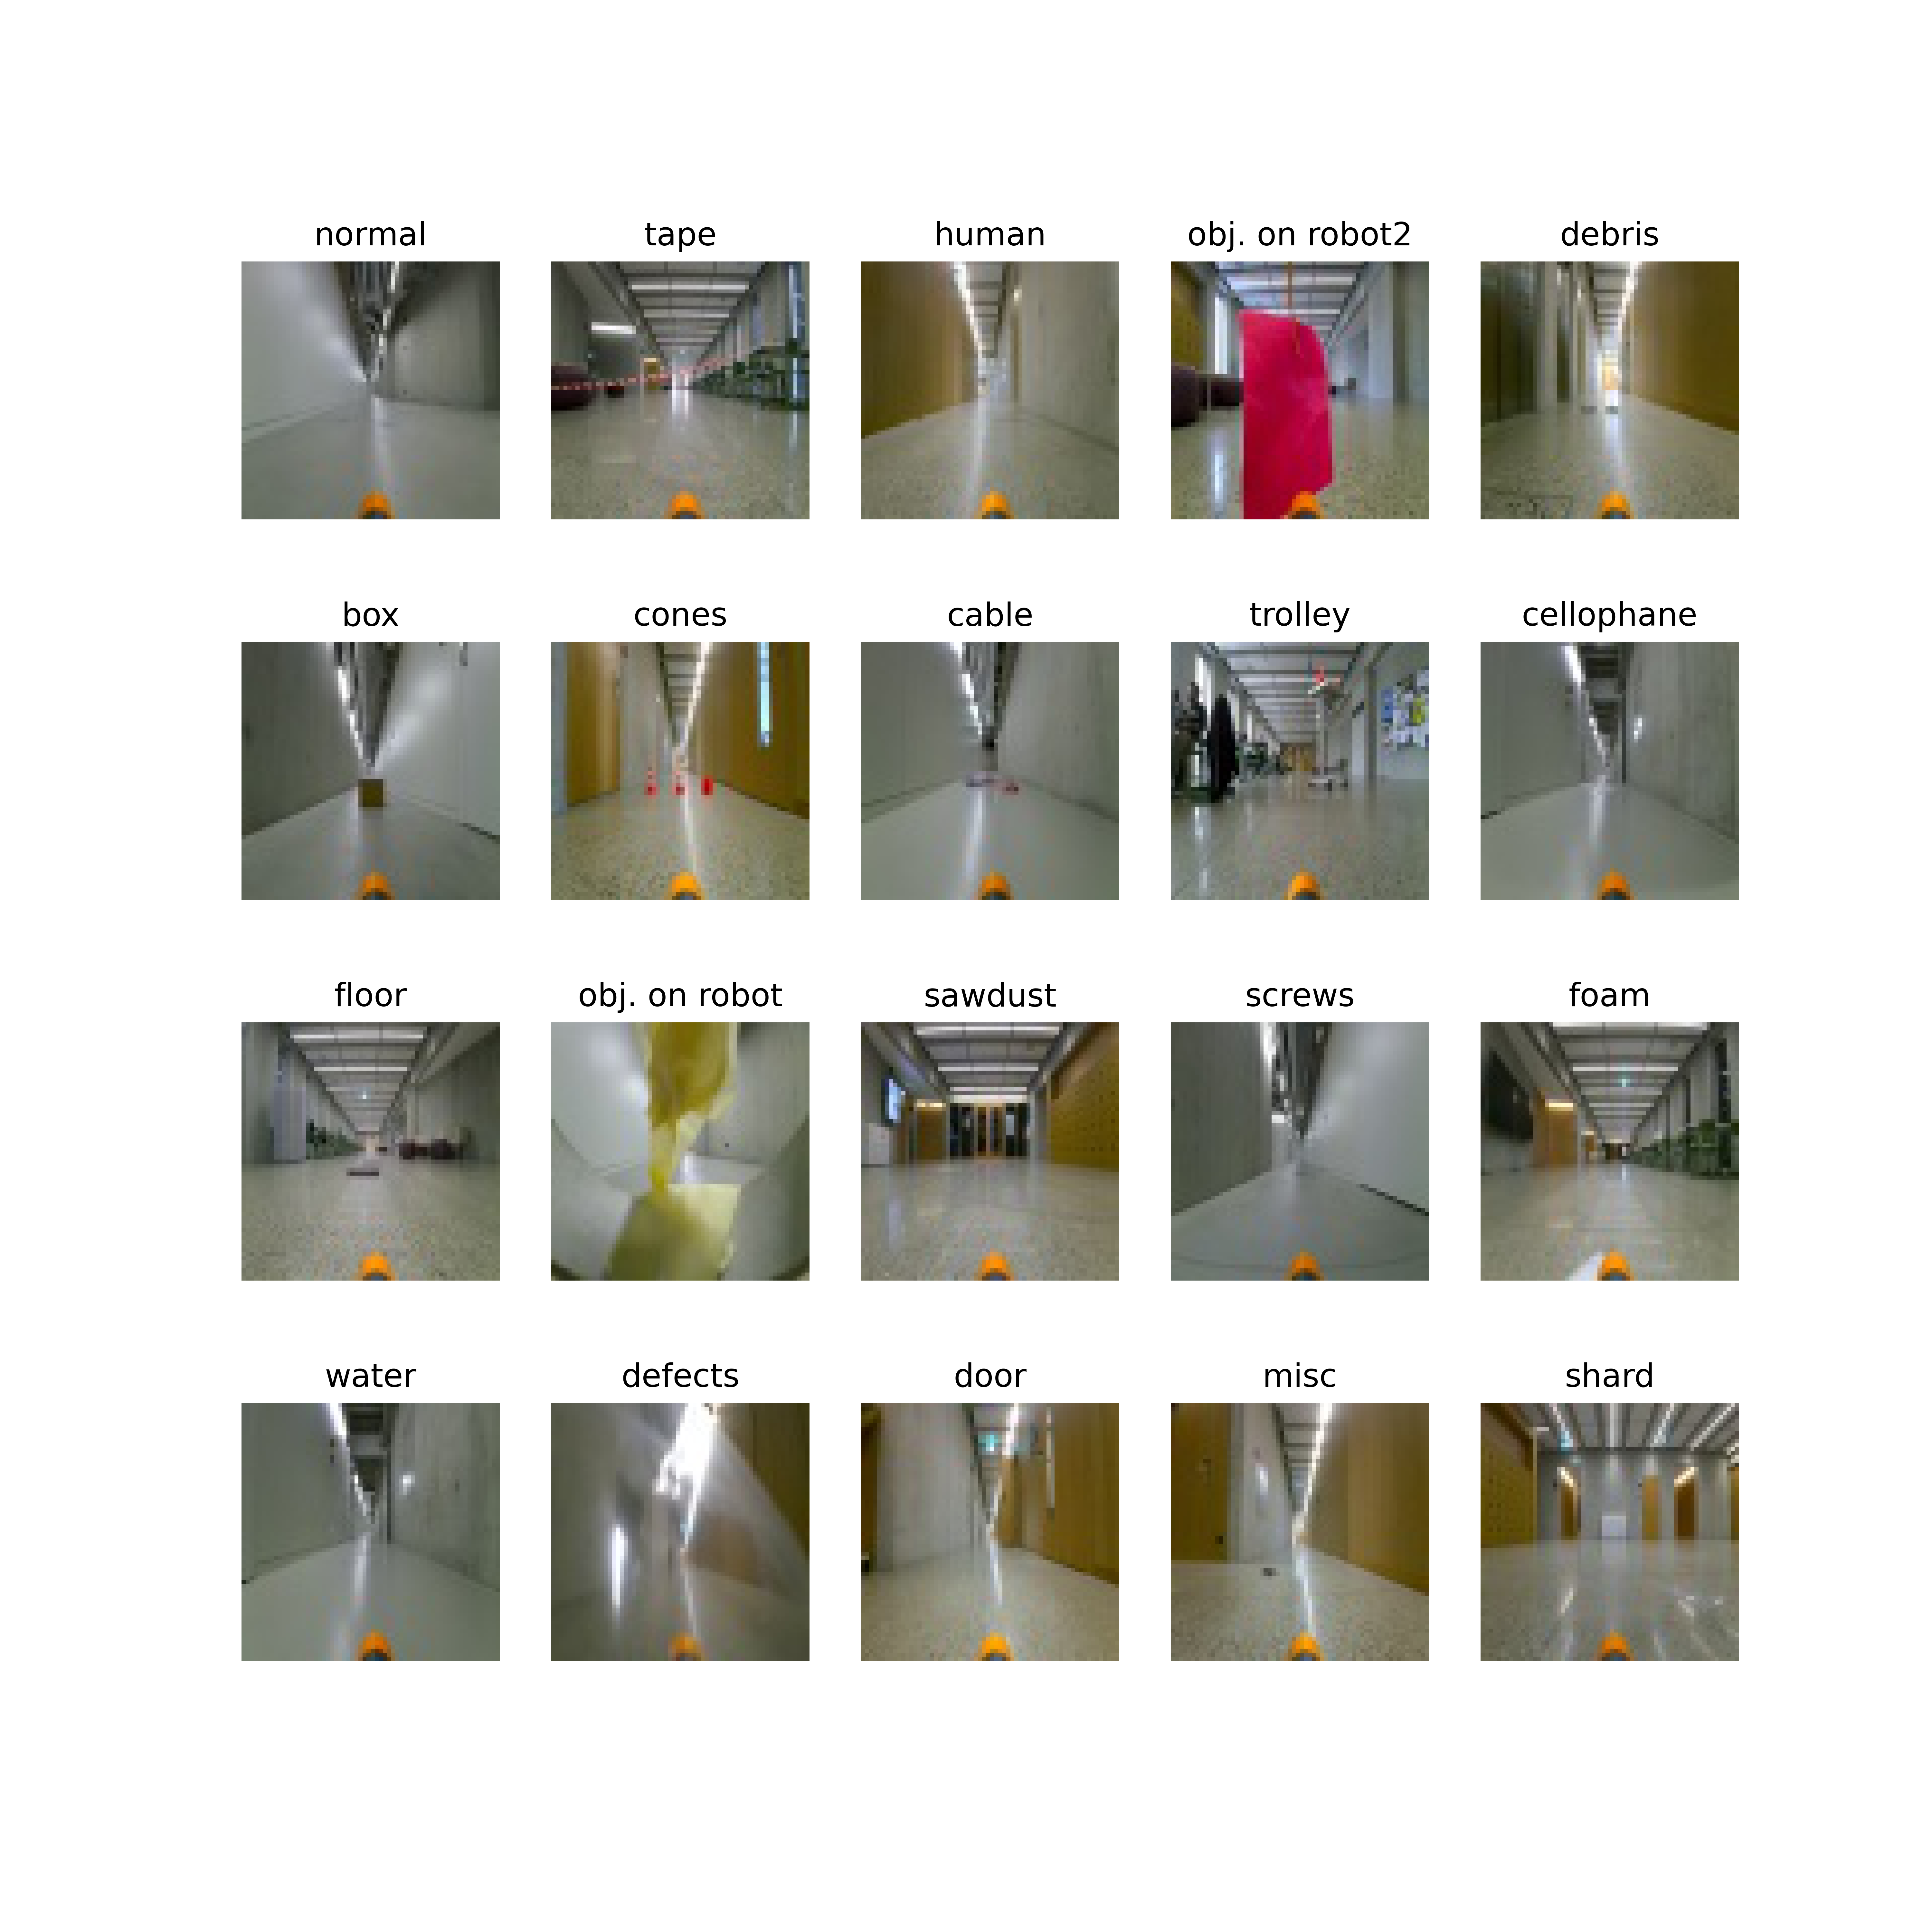
\includegraphics[width=\textwidth]{img/labels/anomalies.png}}
        %         \caption{Robomaster S1, exploded-view from user manual with part names.}
        %         \label{fig:env-ex}
        % \end{figure}
        
        \subsection{Long videos}
        The long videos contain 5 classes. The labels are the following:

        % \begin{itemize}
        %     \item Human
        %     \item Lens dirty
        %     \item Object on Robot
        %     \item Object on Robot 2
        %     \item Normal
        % \end{itemize}

        % \begin{figure}[H]
        %     \centering
        %     \subfloat[]{
        %         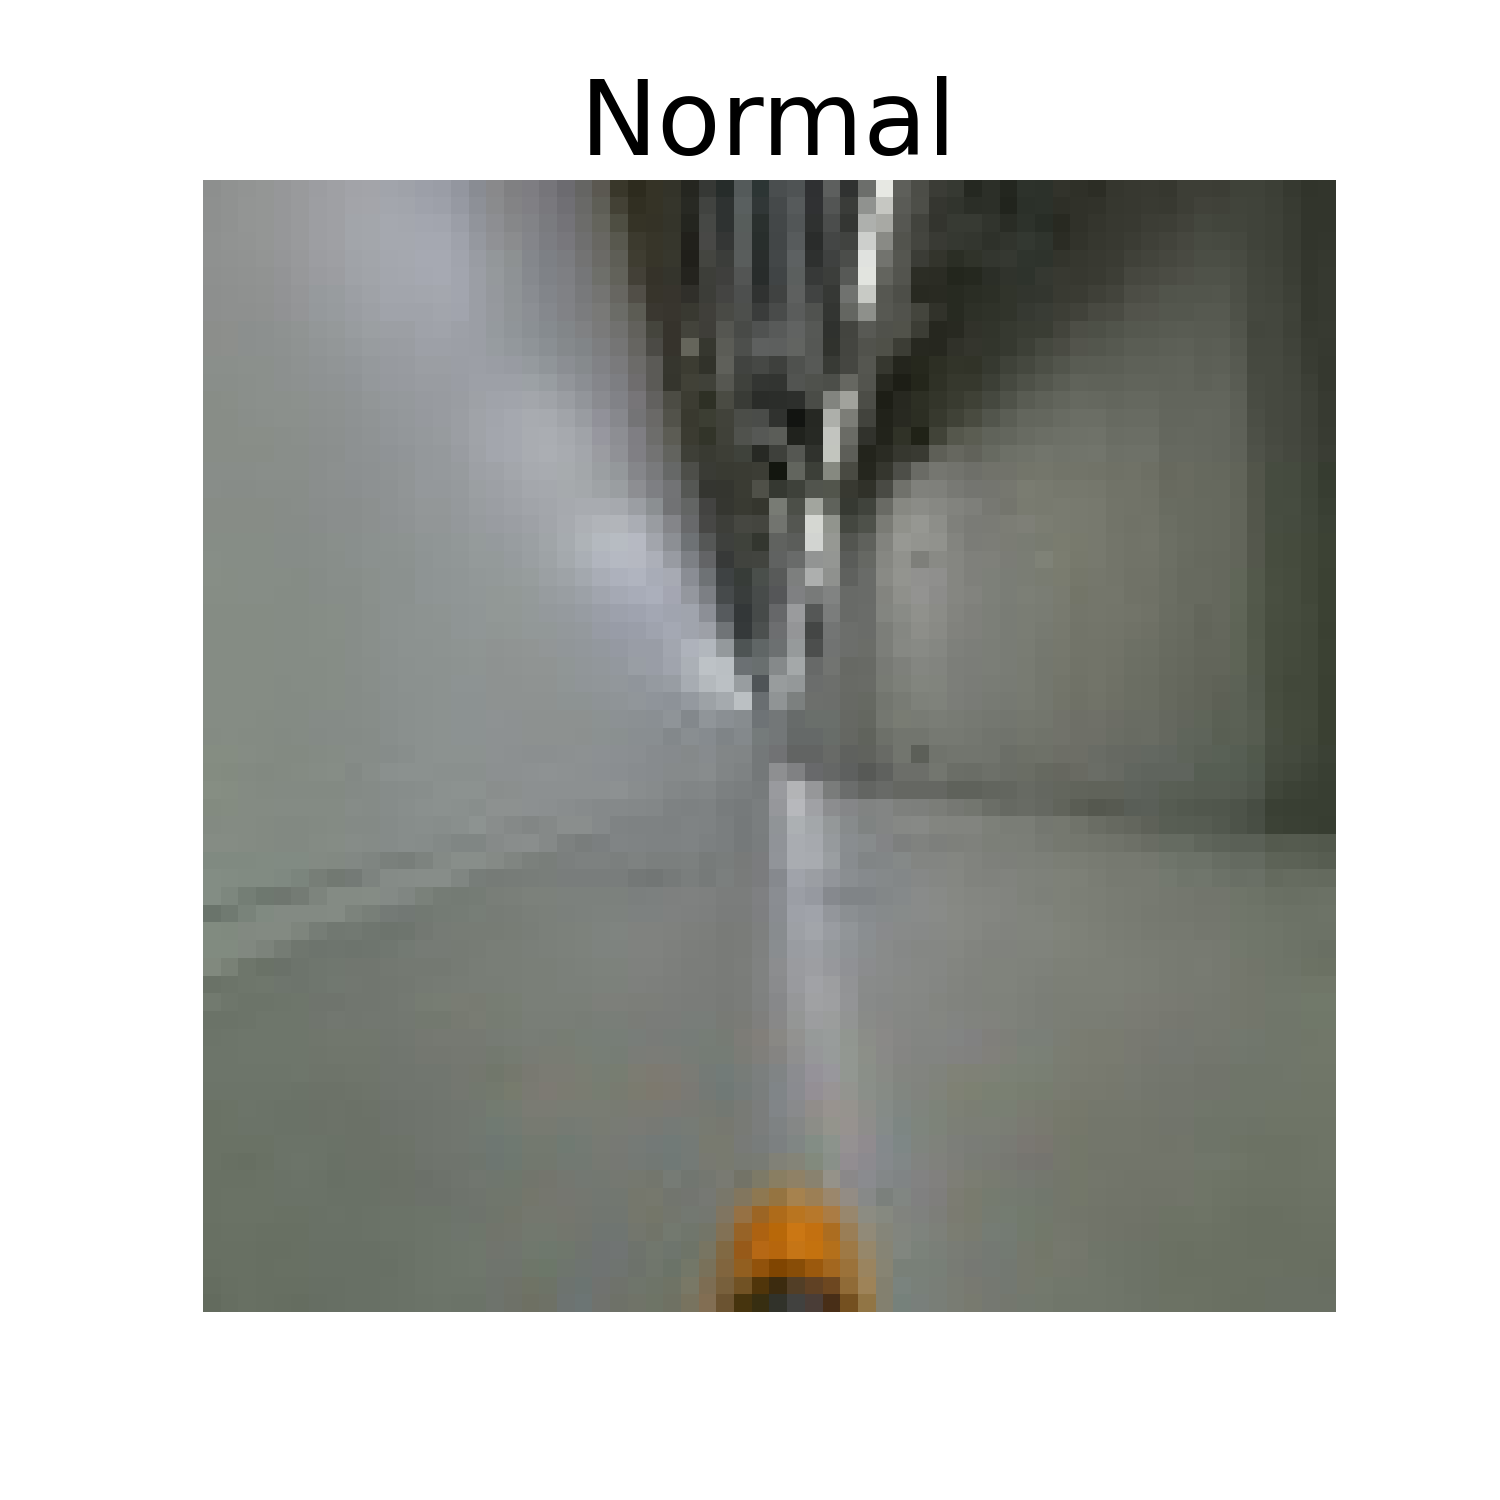
\includegraphics[width=0.3\columnwidth]{img/labels/normal.png}
        %         \label{fig:label-normal}
        %         }
        %     \subfloat[]{
        %         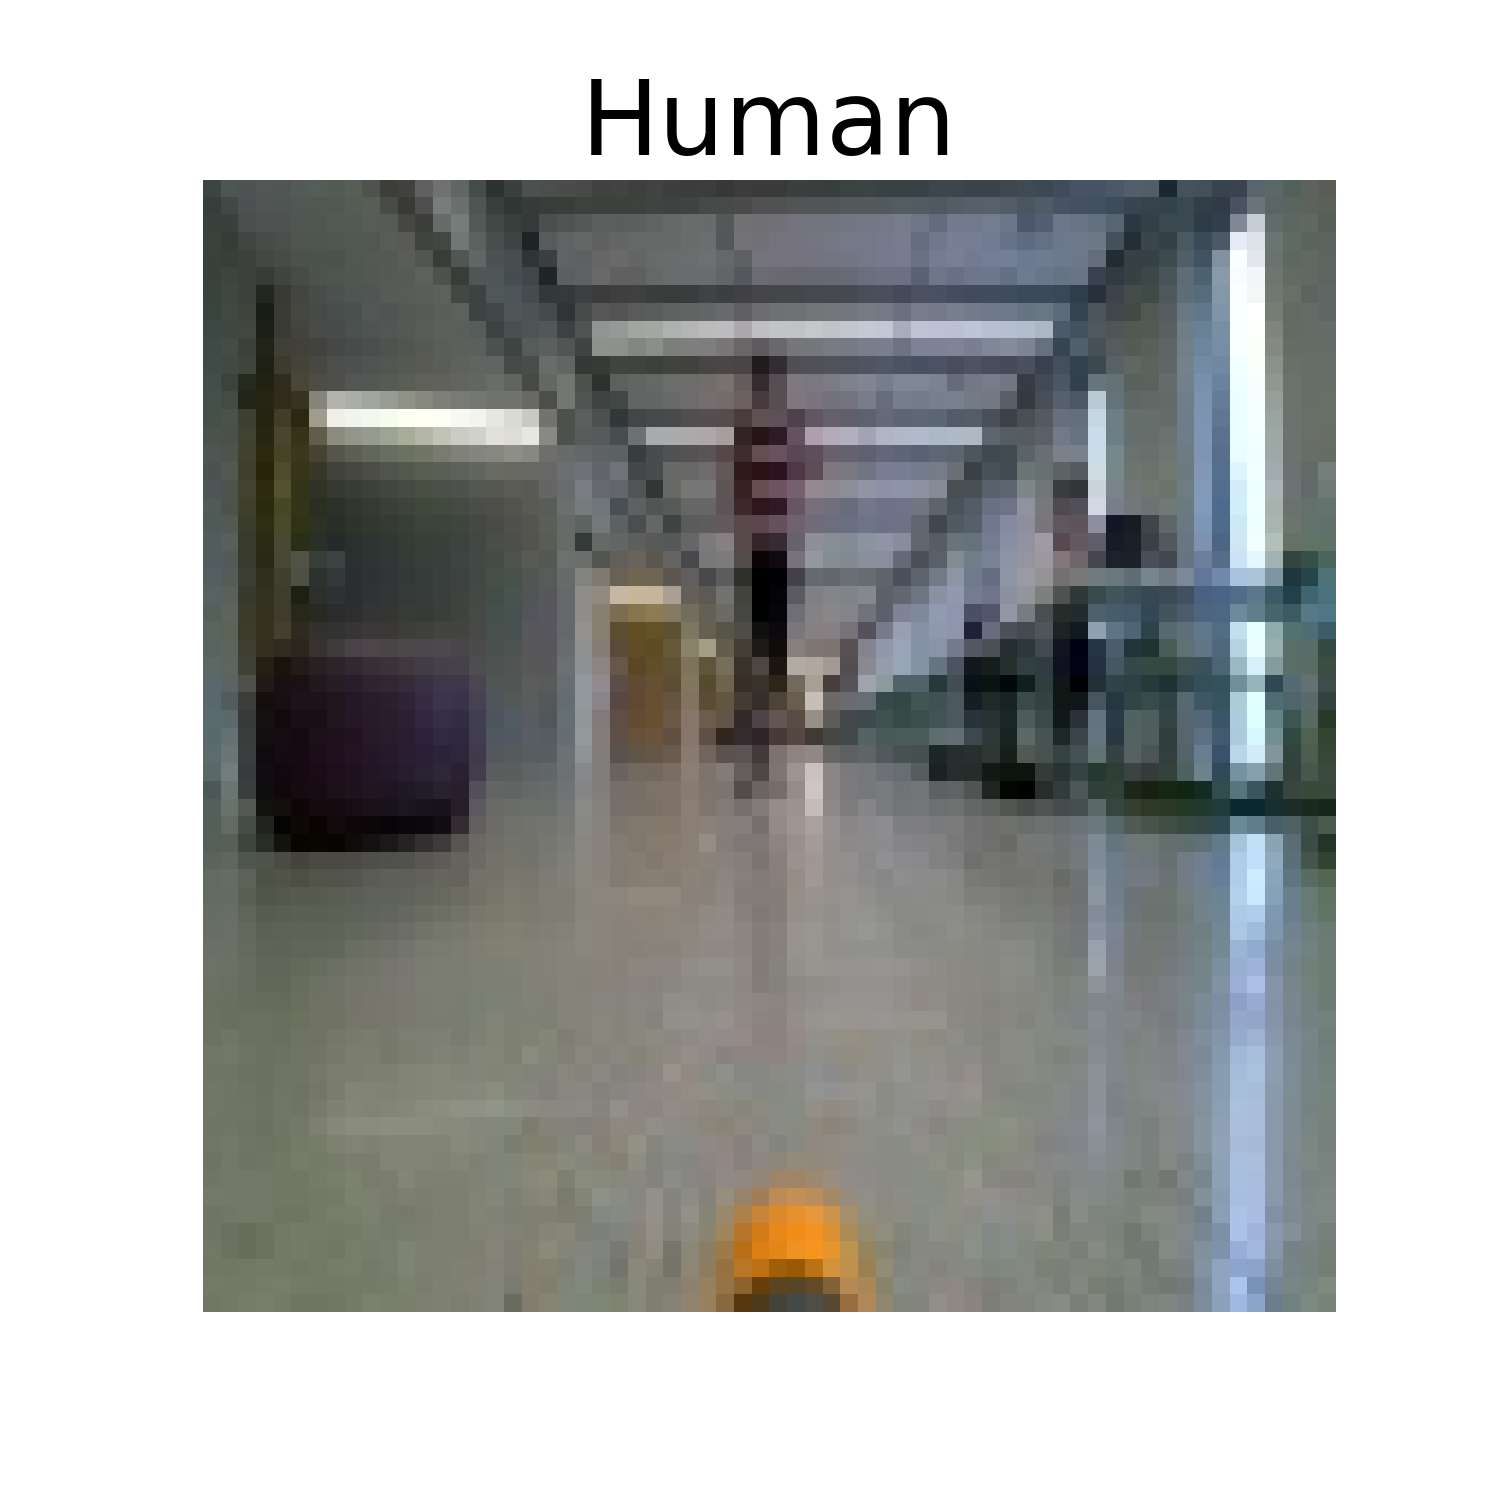
\includegraphics[width=0.3\columnwidth]{img/labels/human.png}
        %         \label{fig:label-human}
        %         }
        %     \subfloat[]{
        %         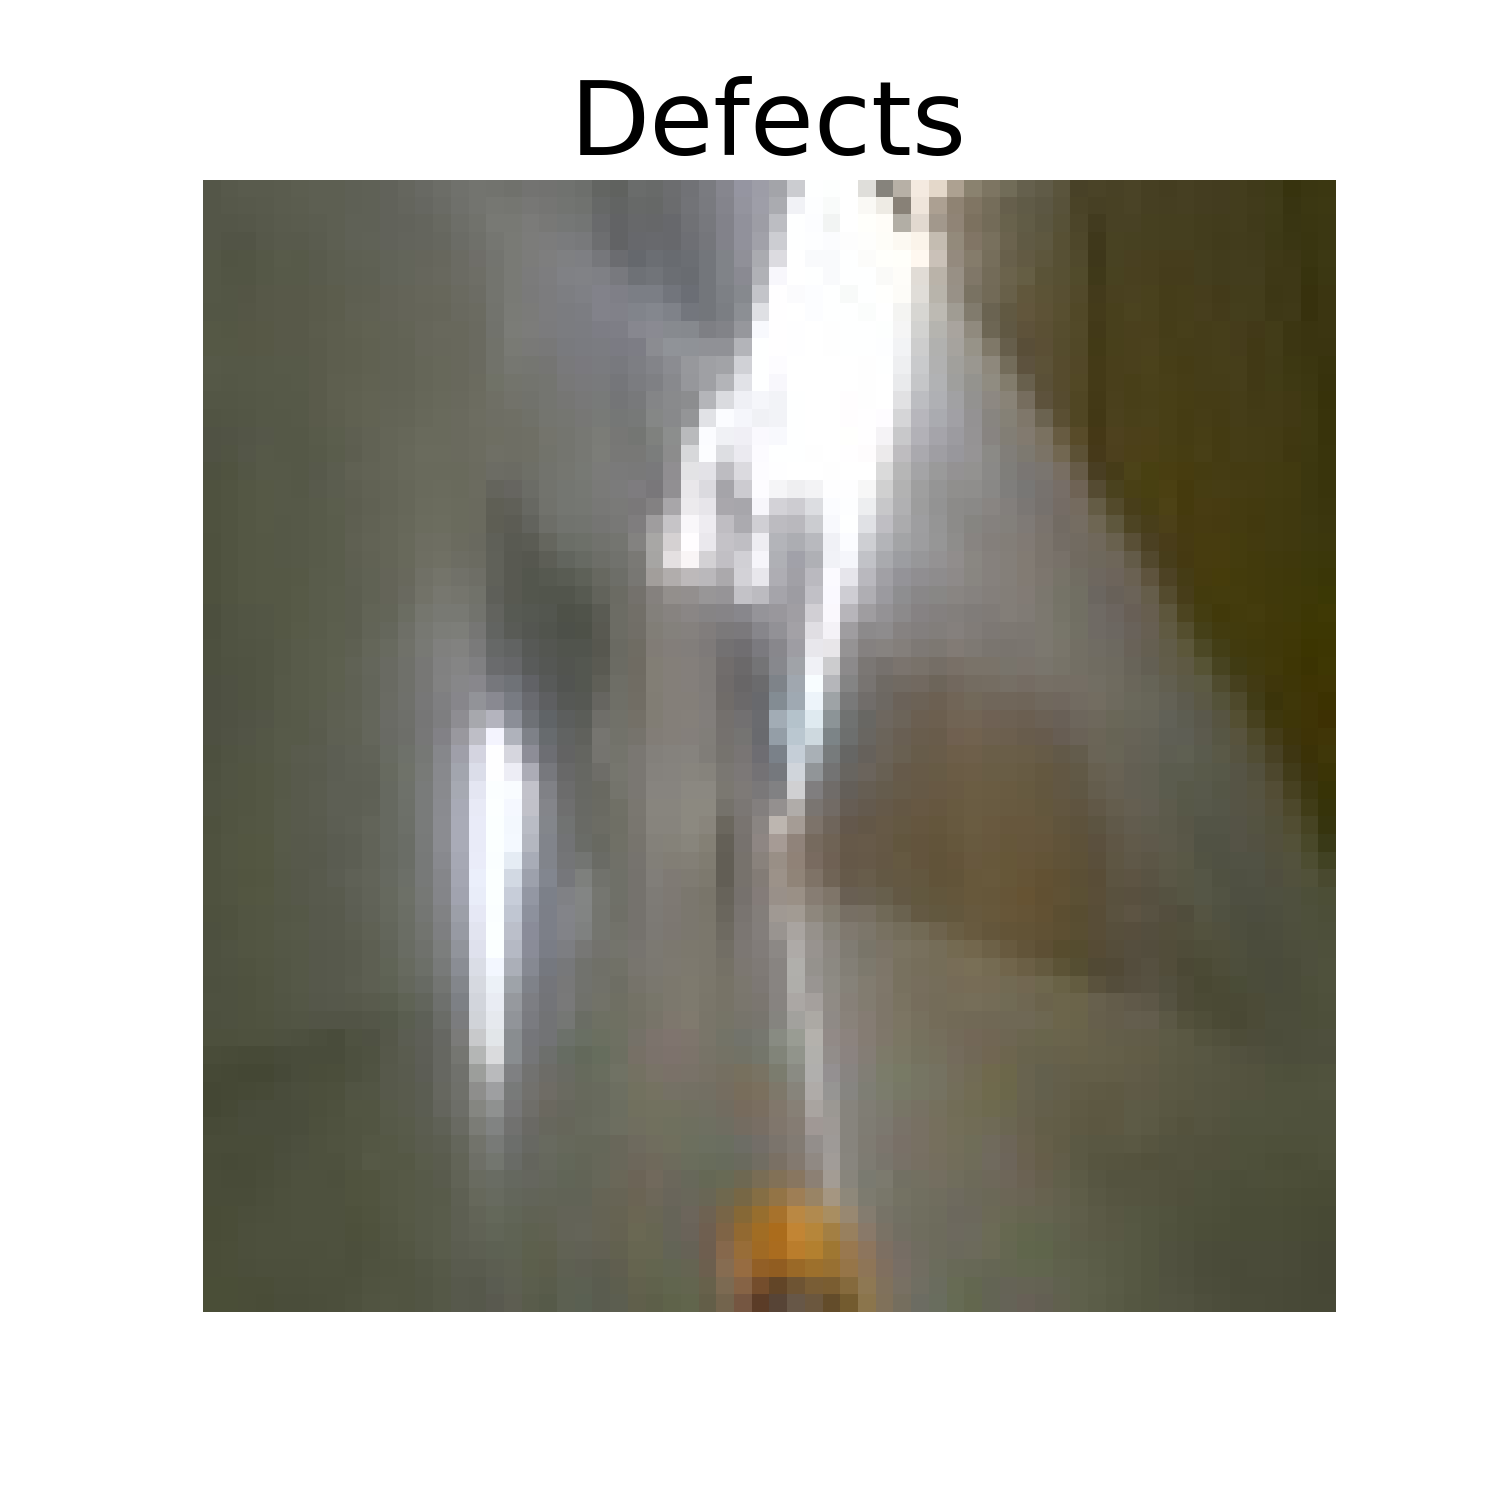
\includegraphics[width=0.3\columnwidth]{img/labels/defects.png}
        %         \label{fig:label-defects}
        %         }
        %     \\
        %     \subfloat[]{
        %         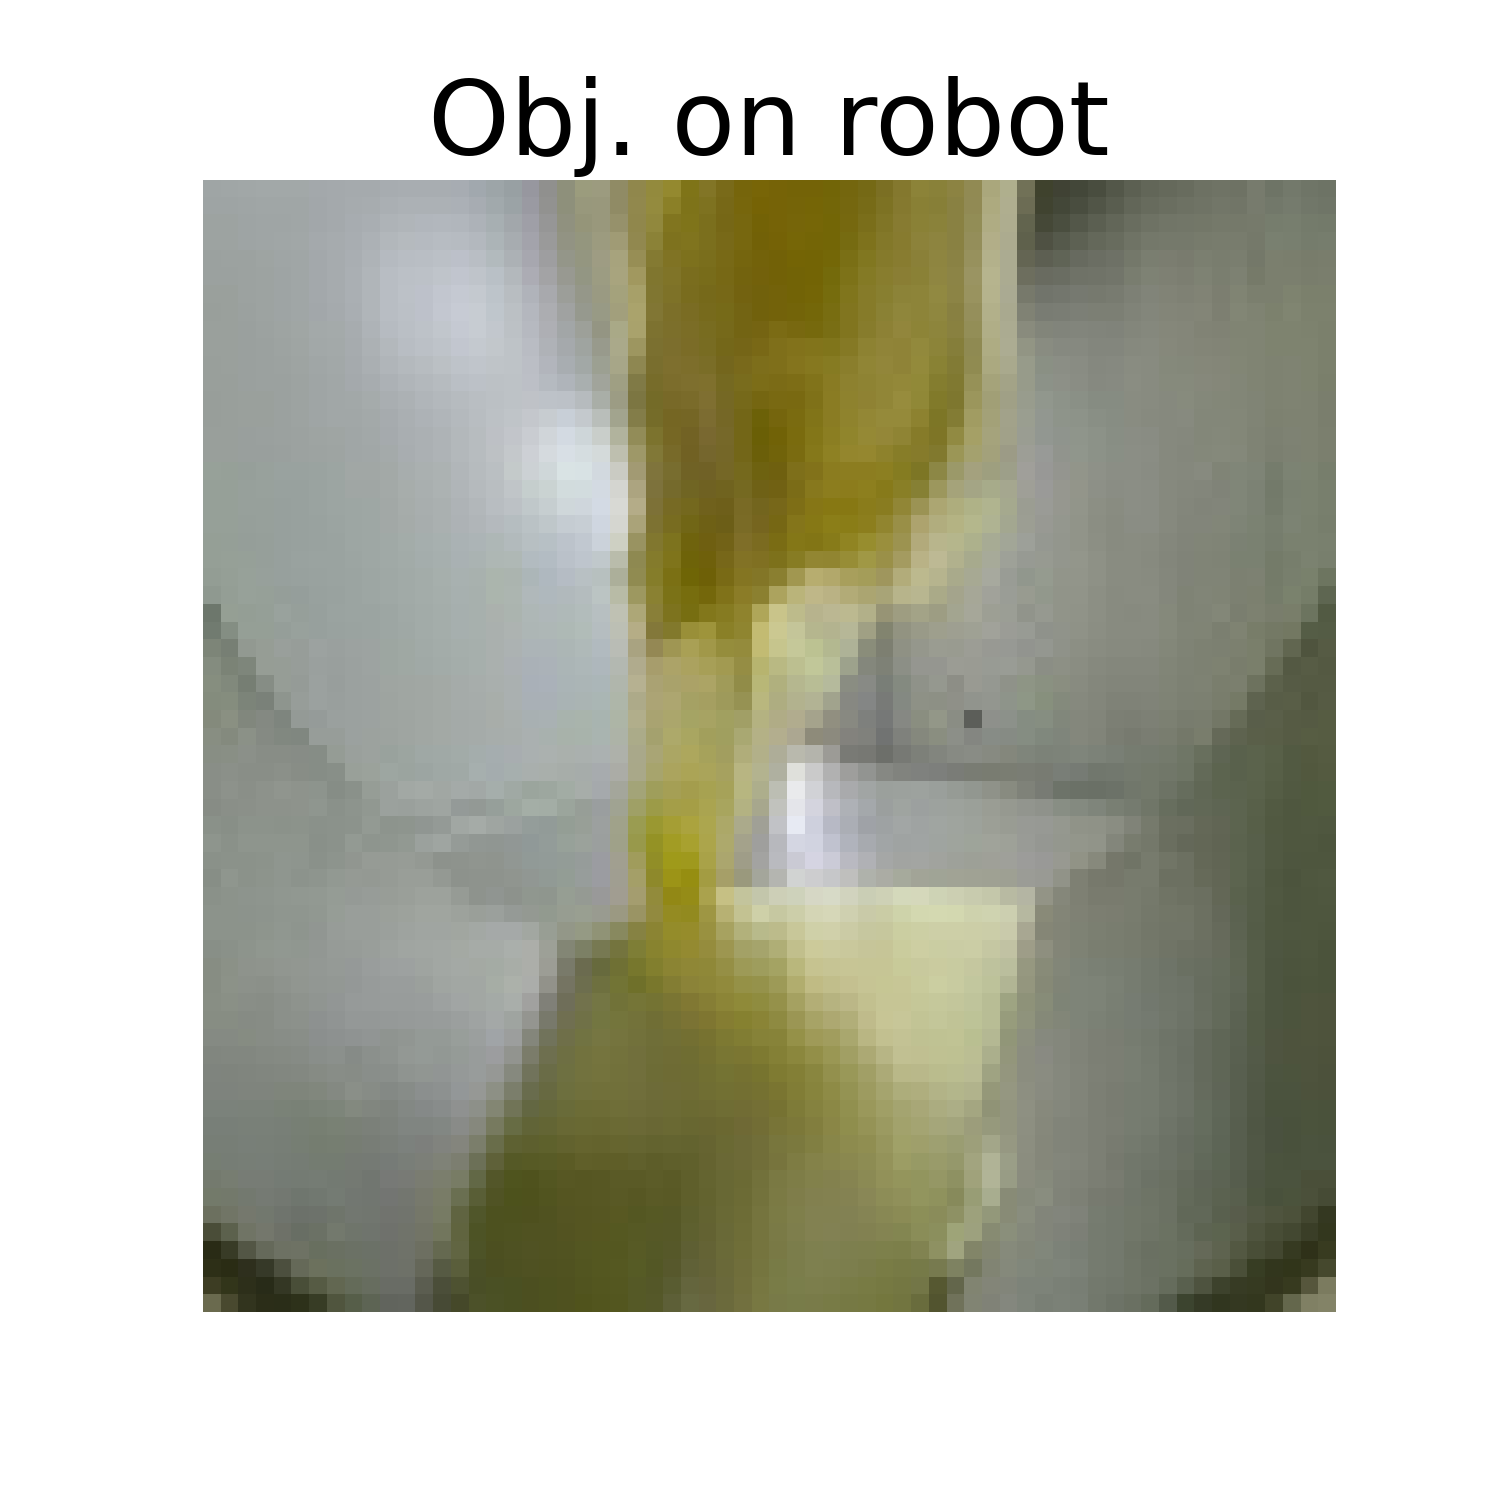
\includegraphics[width=0.3\columnwidth]{img/labels/obj. on robot.png}
        %         \label{fig:label-obj-on-robot}
        %         }
        %     \subfloat[]{
        %         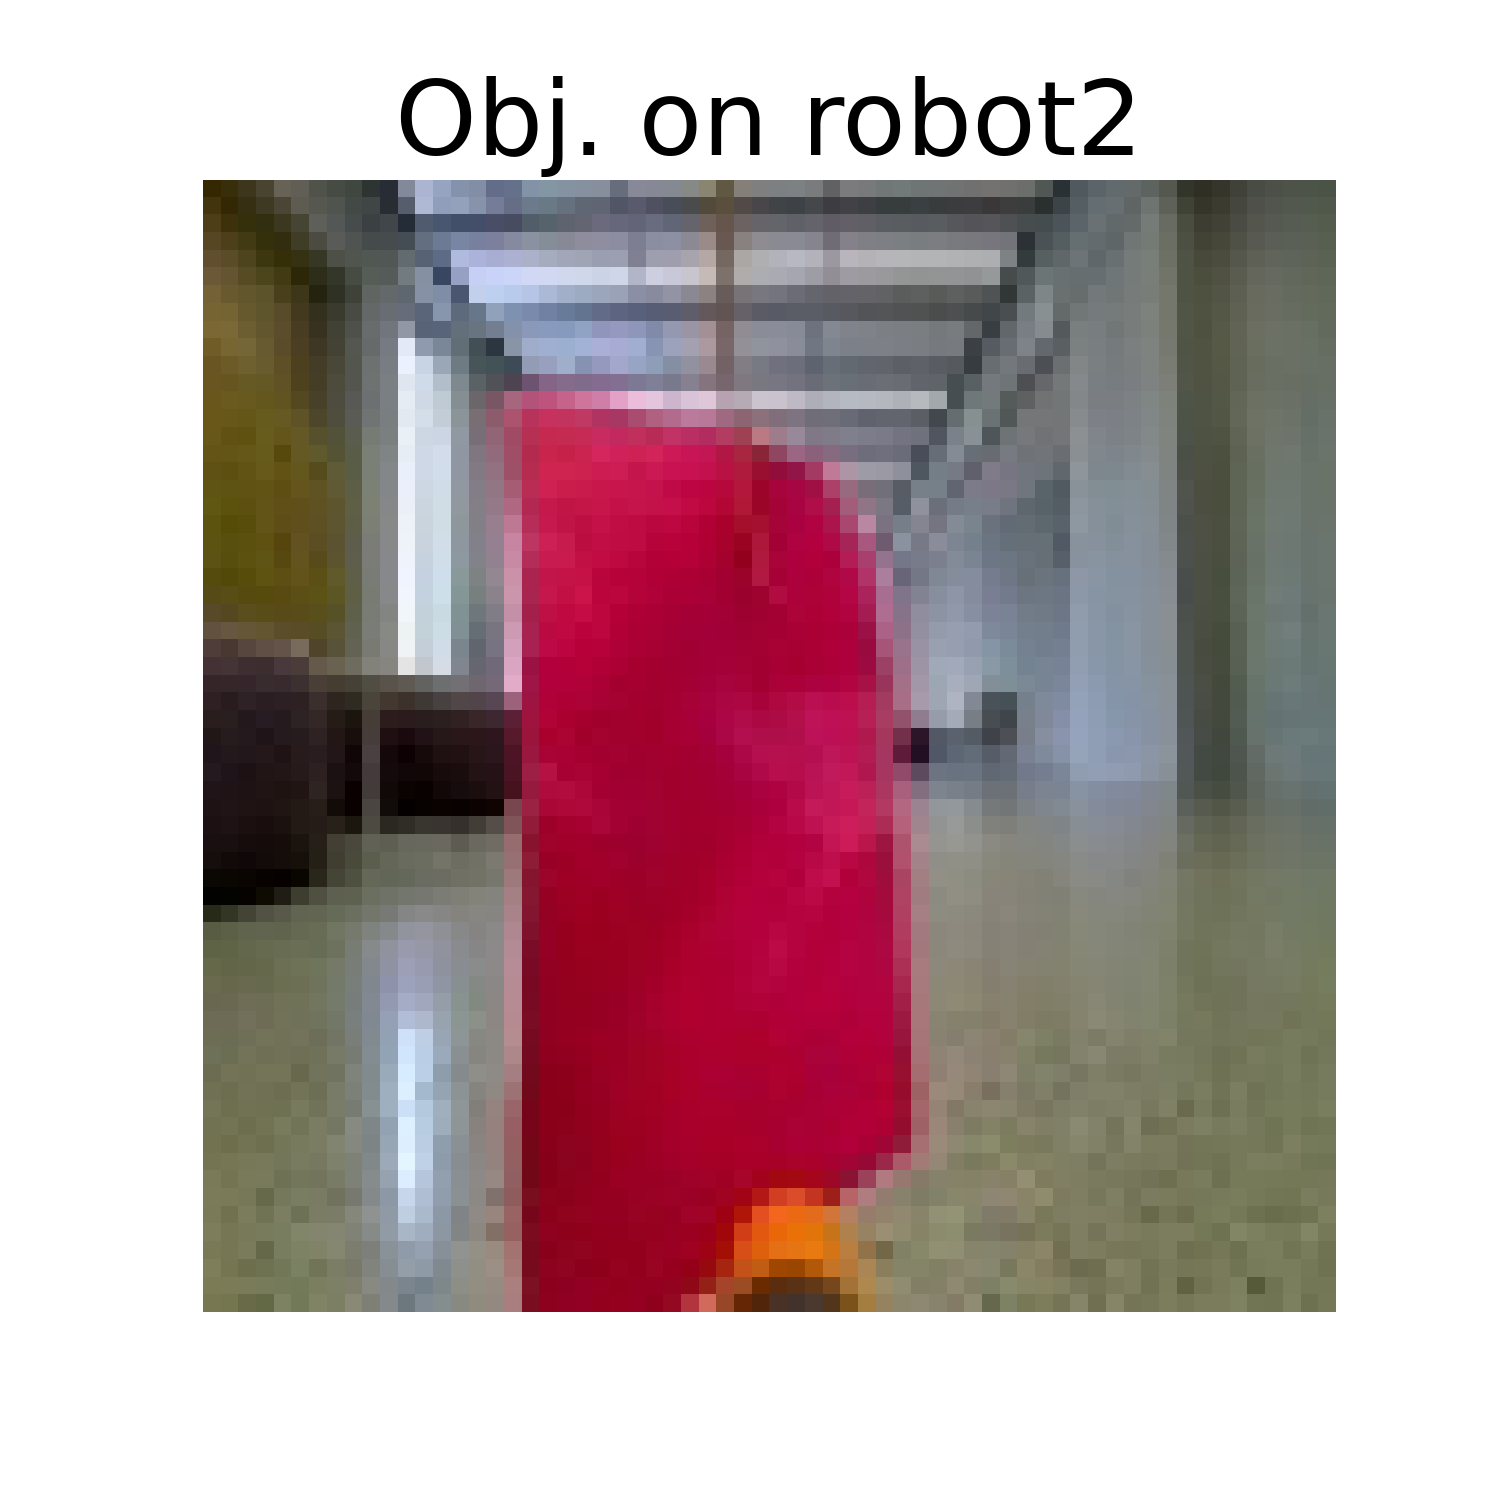
\includegraphics[width=0.3\columnwidth]{img/labels/obj. on robot2.png}
        %         \label{fig:label-obj-on-robot2}
        %         }
        %     \caption{Images for each corresponding label of the long section of the dataset}
        %     \label{fig:labels-long}
        % \end{figure}

        \subsubsection*{Normal}
            The normal class (\autoref{fig:label-normal}) contains frames where the camera is not obstructed by any object. The camera is clean and the robot's path is not obstructed.
            \begin{figure}[H]
                \centering
                \centerline{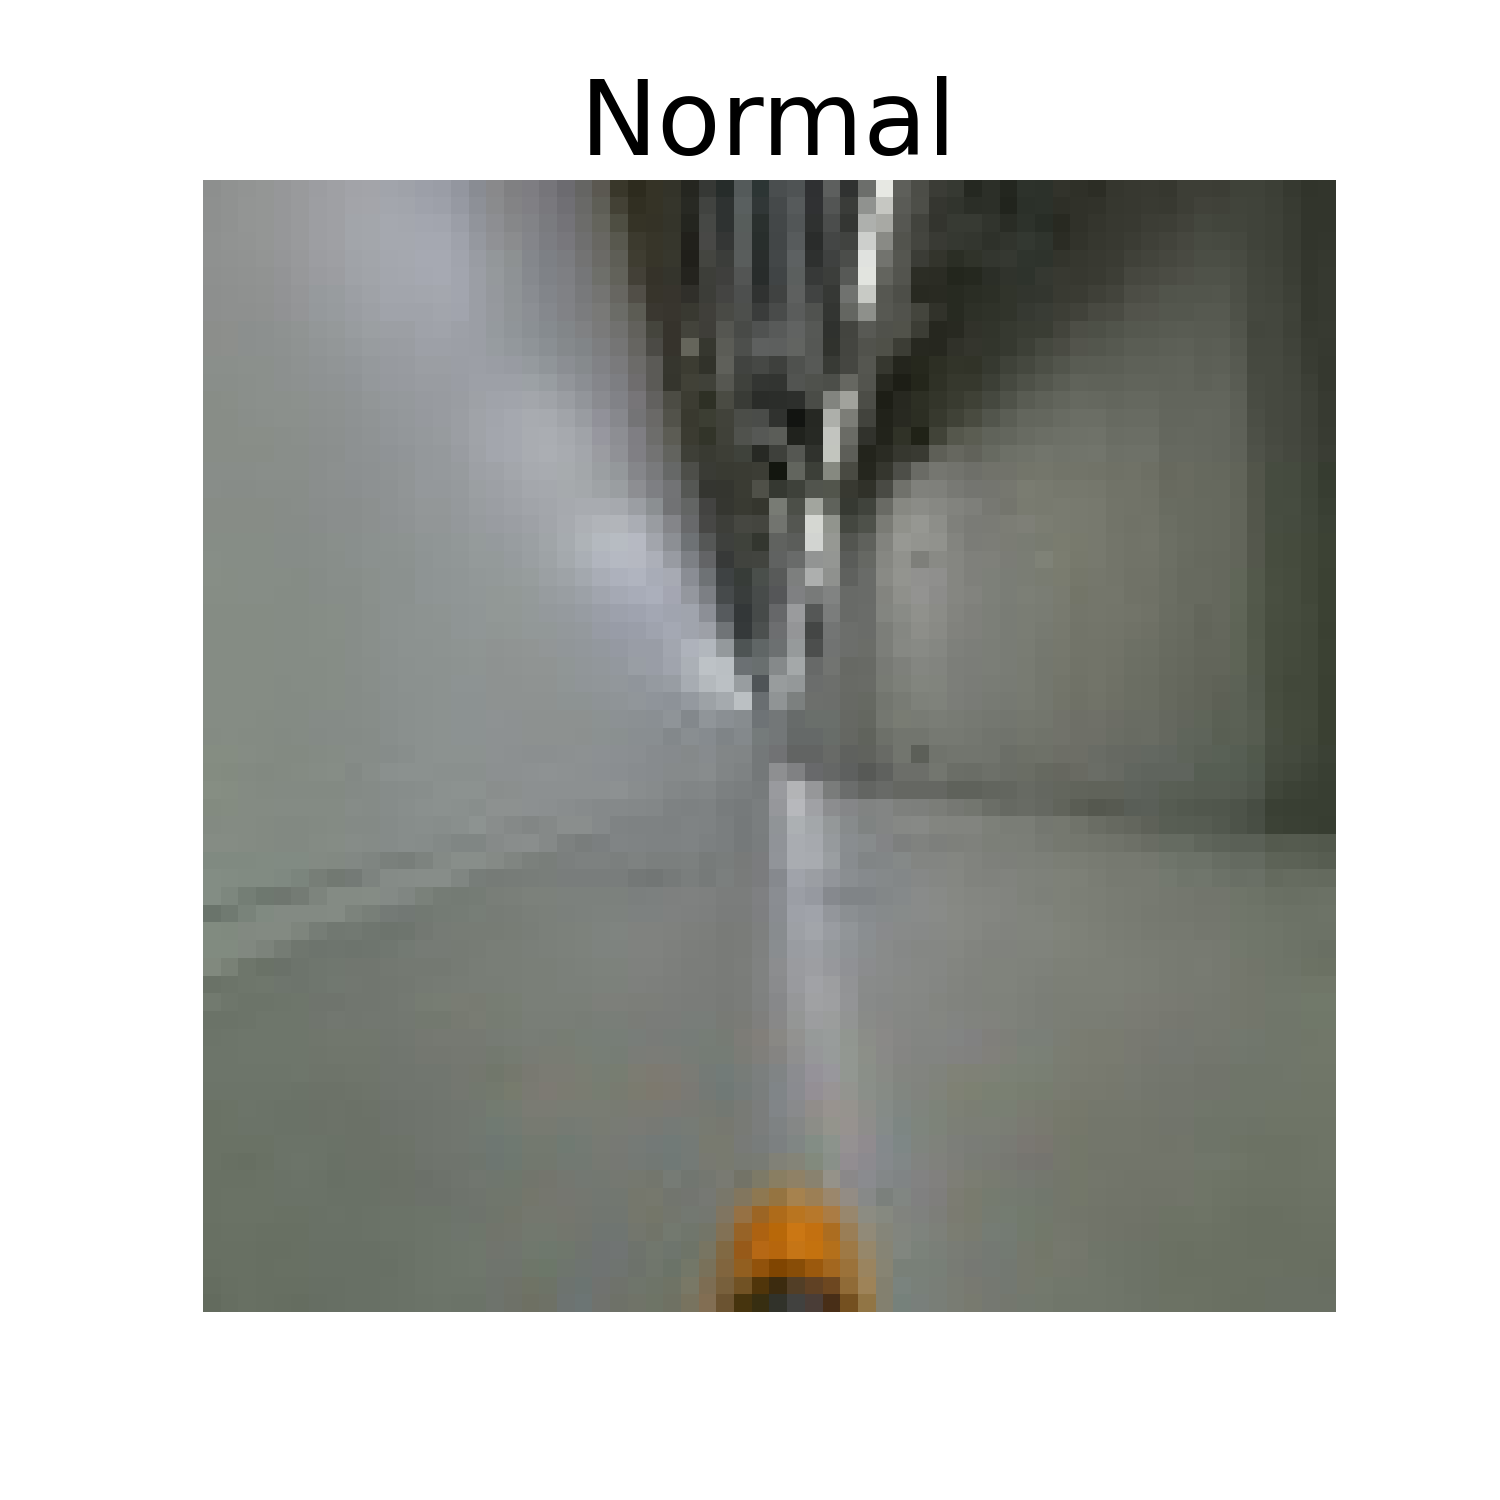
\includegraphics[width=0.75\textwidth]{img/labels/normal.png}}
                \caption{Robots\&Hazards dataset Corridors scenario, label normal}
                \label{fig:label-normal}
            \end{figure}

        \subsubsection*{Human}
            The human class (Figure \autoref{fig:label-human}) contains frames where a person is obstructing the robot's path. The person is usually standing in front of the robot and moves in the same direction as the robot.
            \begin{figure}[H]
                \centering
                \centerline{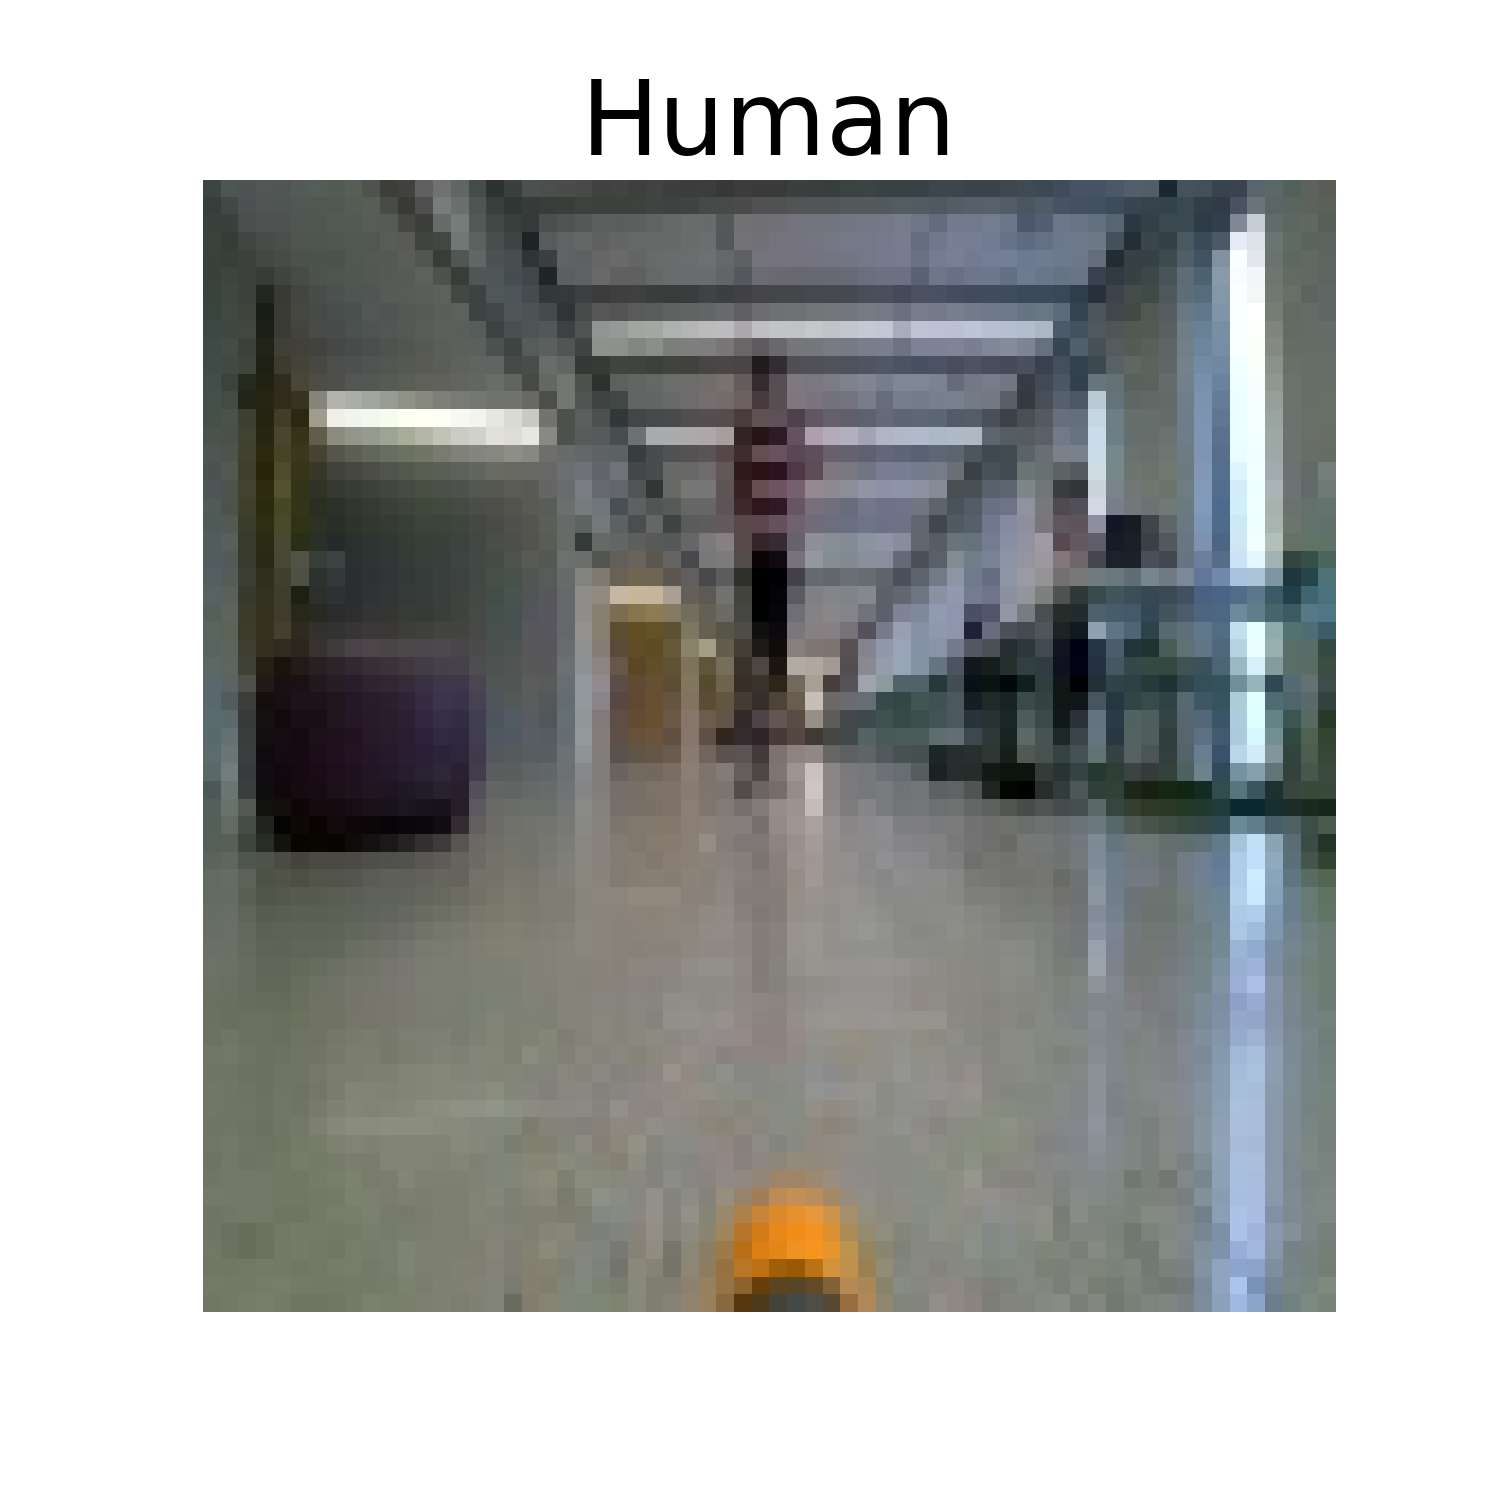
\includegraphics[width=0.75\textwidth]{img/labels/human.png}}
                \caption{Robots\&Hazards dataset Corridors scenario, label human}
                \label{fig:label-human}
            \end{figure}

        \subsubsection*{Defects}
            The defects class (\autoref{fig:label-defects}) contains frames where the camera has some kind of defect. The defect can be a scratch, a stain, or a fingerprint on the lens. This anomaly is simulated by placing an antistatic bag on the camera.
            \begin{figure}[H]
                \centering
                \centerline{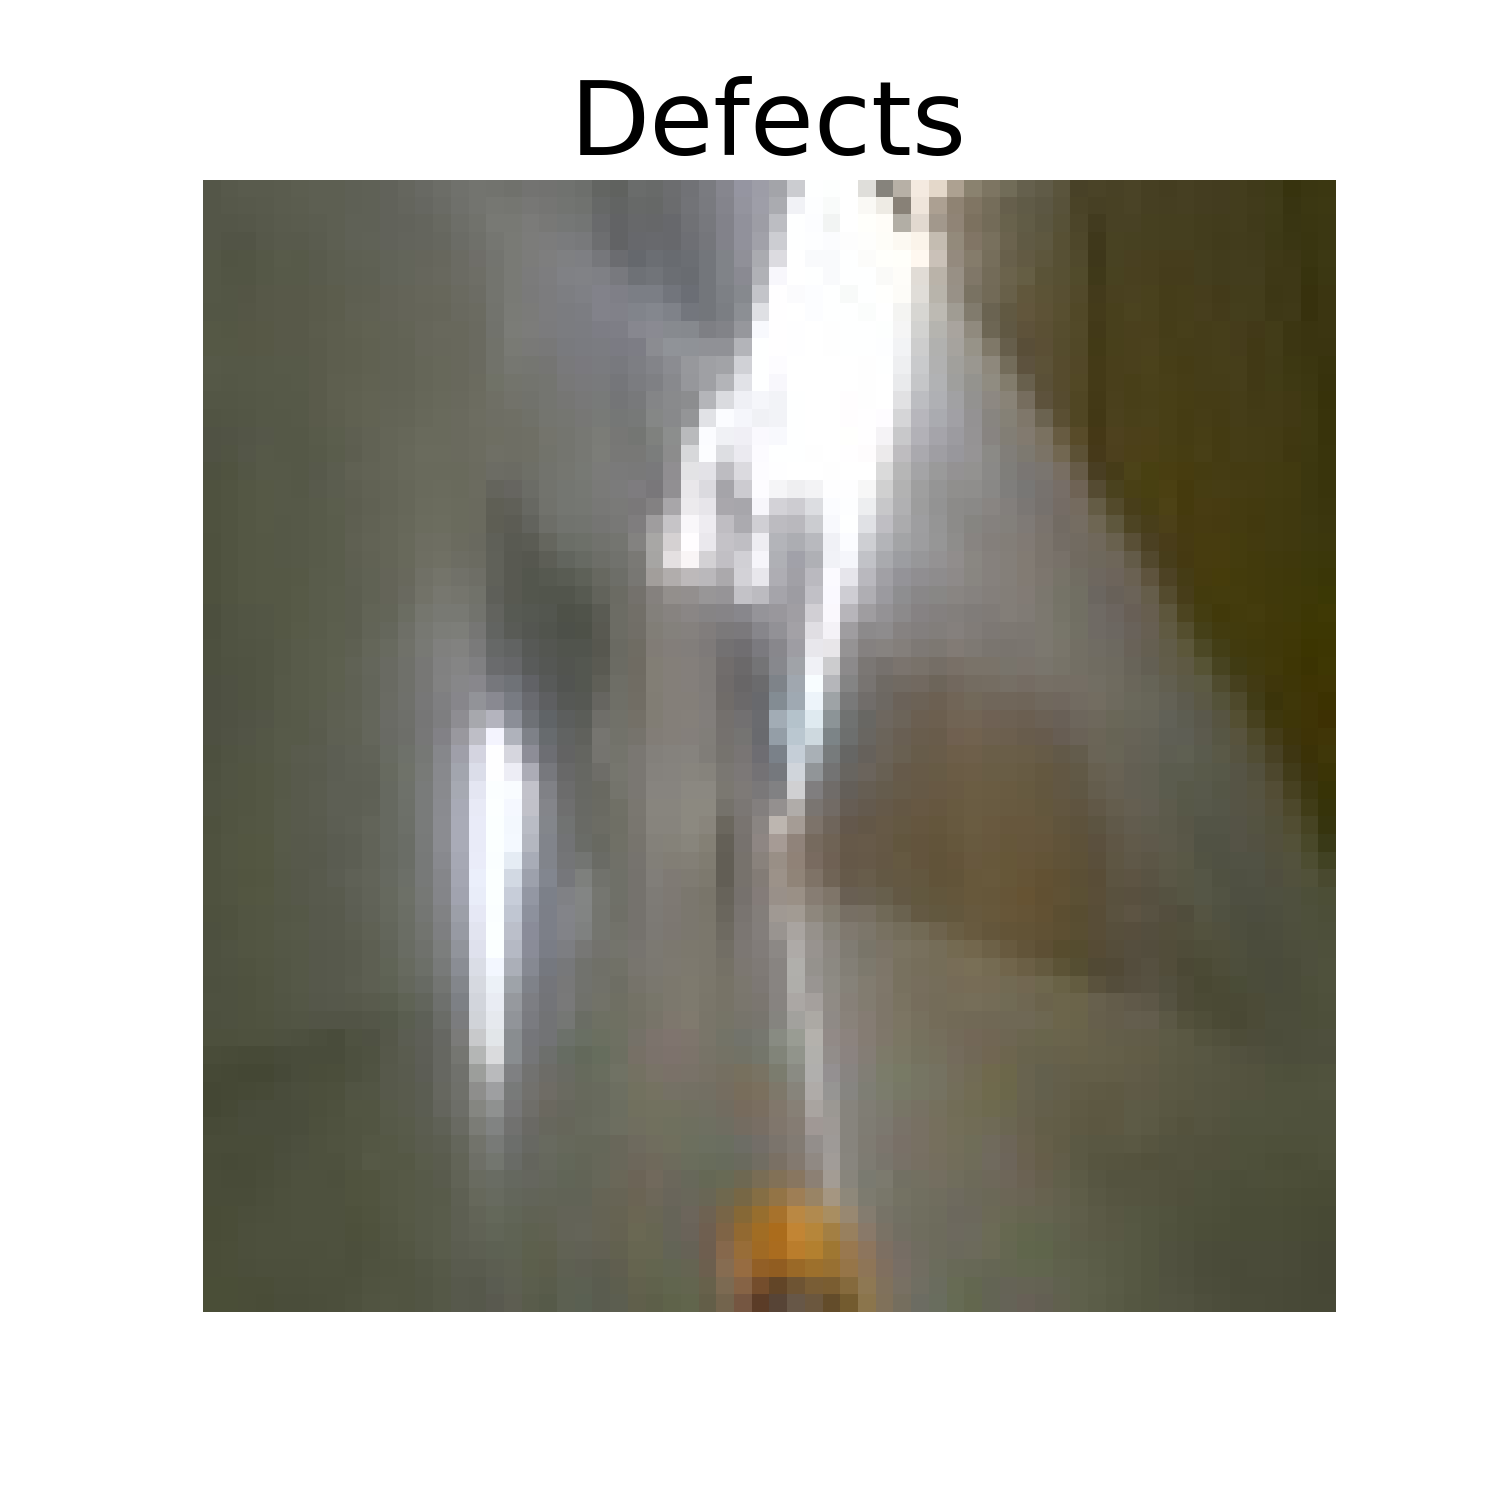
\includegraphics[width=0.75\textwidth]{img/labels/defects.png}}
                \caption{Robots\&Hazards dataset Corridors scenario, label defects}
                \label{fig:label-defects}
            \end{figure}

        \subsubsection*{Object on Robot}
            The object on robot class (\autoref{fig:label-obj-on-robot}) contains frames where the robot \acrshort{fov} is obstructed by some kind of object fallen and stuck over the camera. \autoref{fig:sampei} shows the robot with the anomaly mounted on it.
            
             \begin{figure}[H]
                \centering
                \centerline{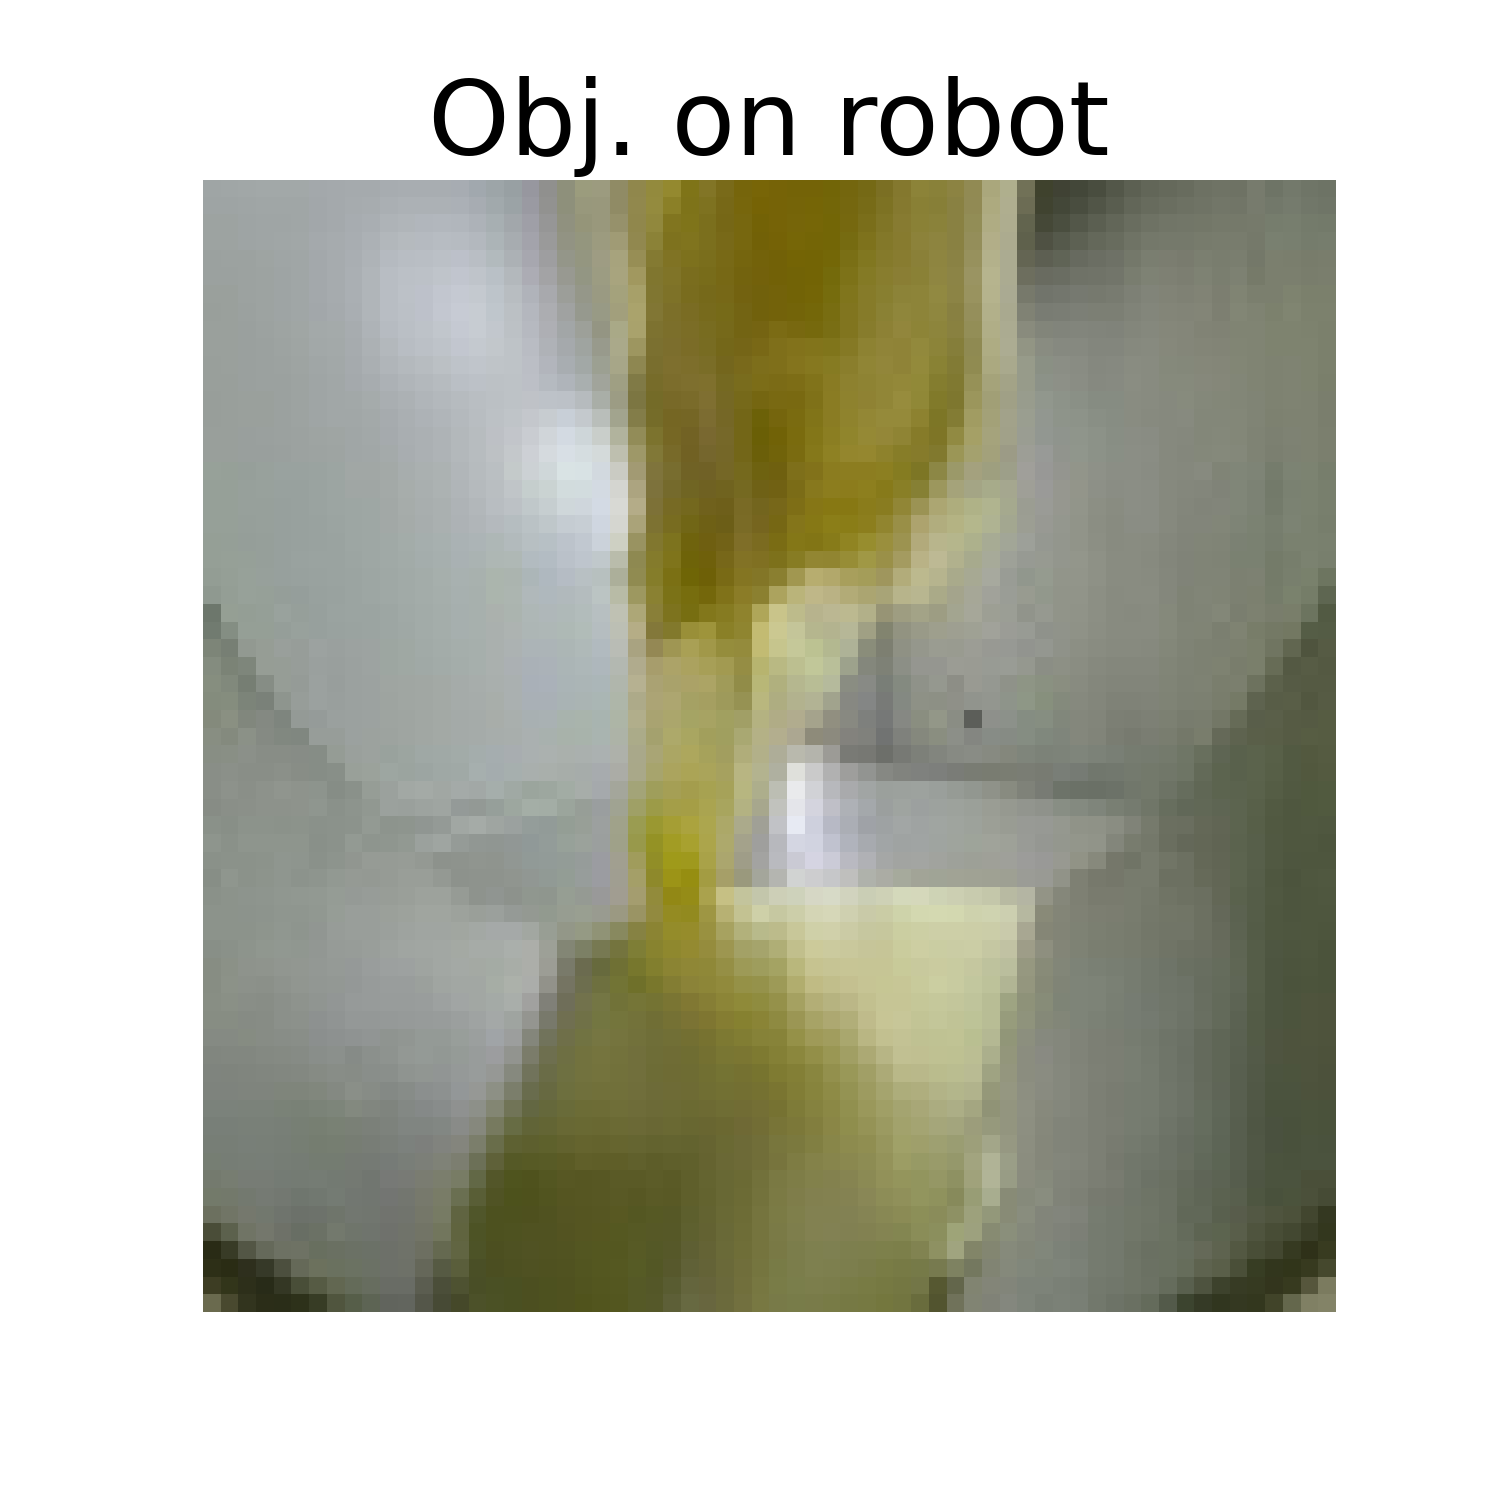
\includegraphics[width=0.75\textwidth]{img/labels/obj. on robot.png}}
                \caption{Robots\&Hazards dataset Corridors scenario, label Object on Robot}
                \label{fig:label-obj-on-robot}
            \end{figure}
            
            \begin{figure}[H]
                \centering
                \centerline{\includegraphics[width=\textwidth]{img/obj2_t.png}}
                \caption{Robomaster S1 mounted with the Object on robot anomaly}
                \label{fig:sampei}
            \end{figure}

        \subsubsection*{Object on Robot 2}
            This class is similar to the previous one, but the object is placed on the robot differently. The object is placed further in the camera in a way to only obstruct the central part of the robot's \acrshort{fov}. In \autoref{fig:sampei2} we can see the robot with the anomaly mounted on.
            \begin{figure}[H]
                \centering
                \centerline{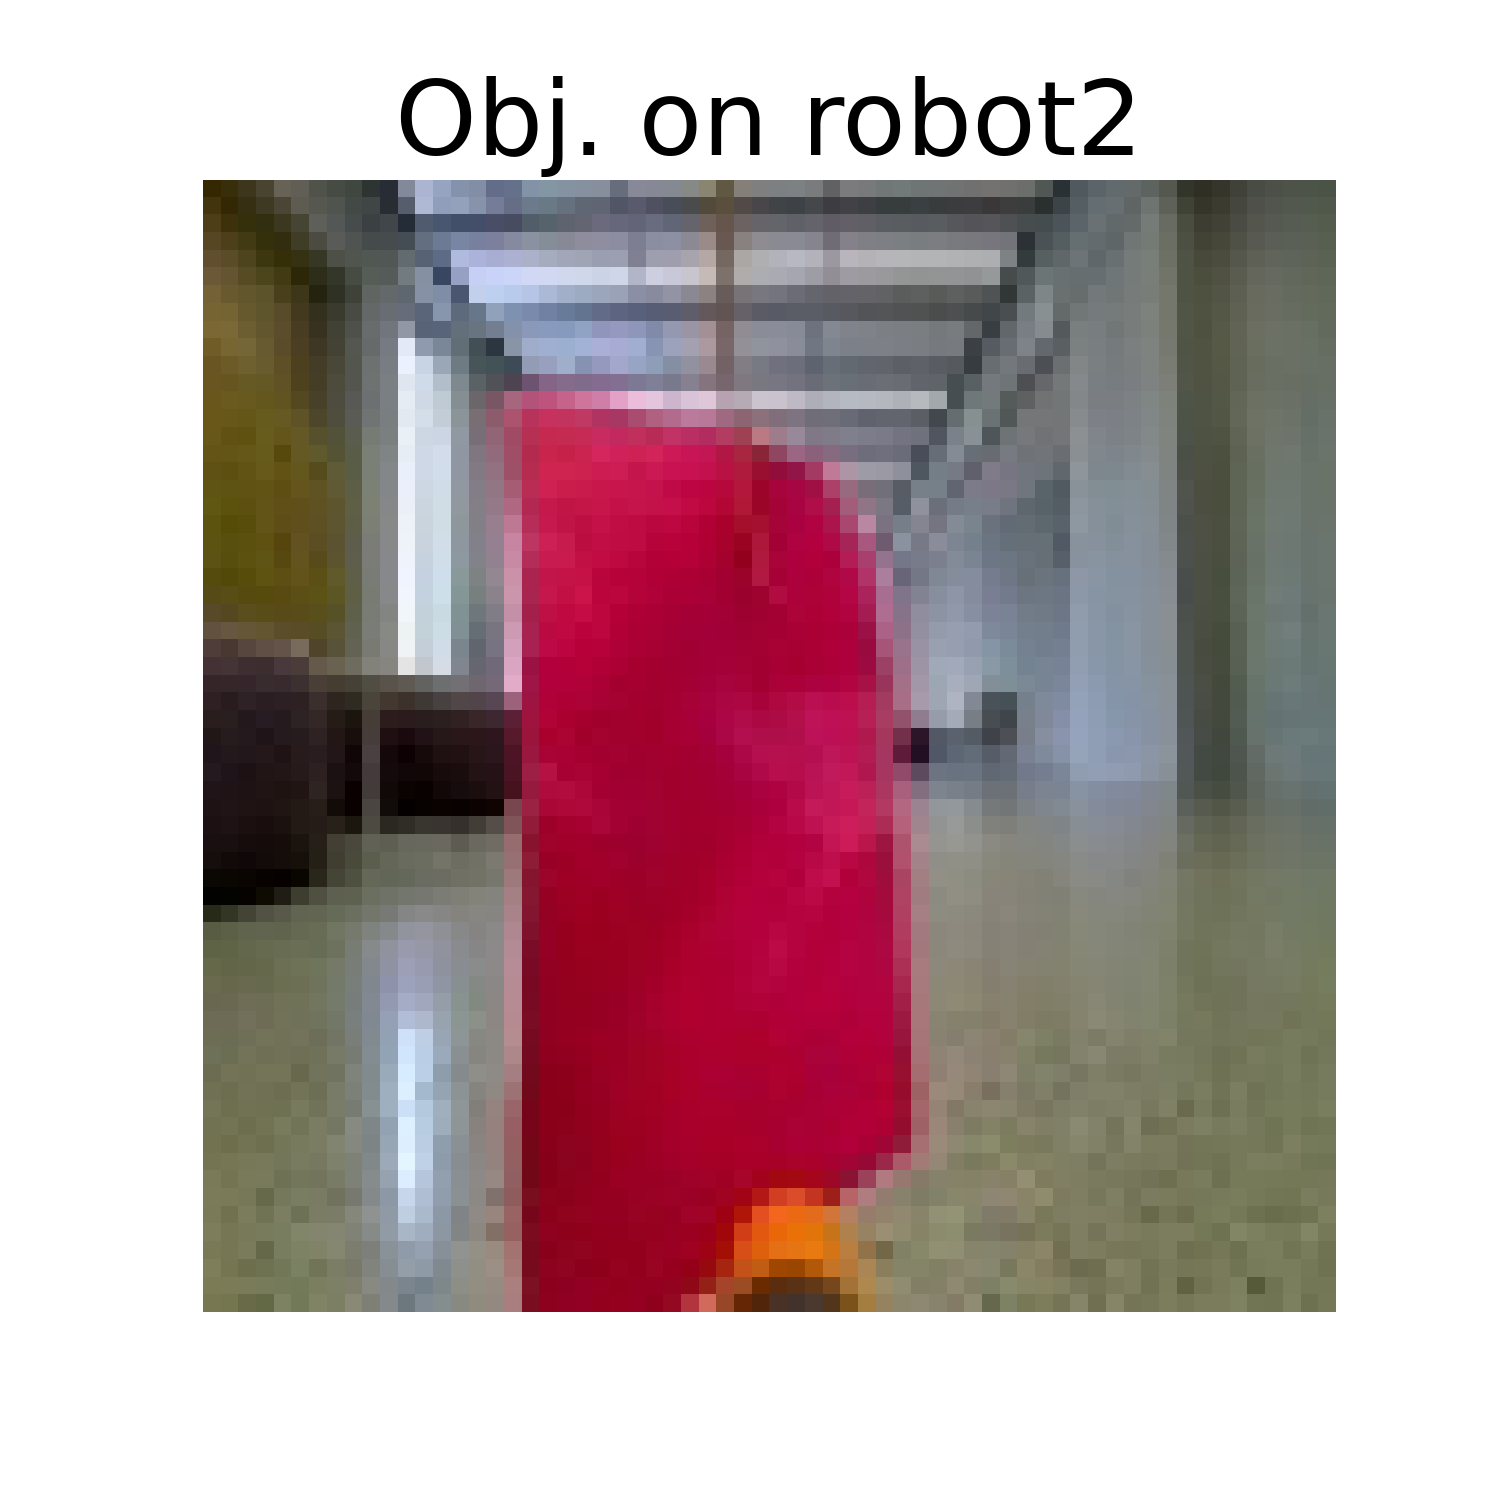
\includegraphics[width=0.75\textwidth]{img/labels/obj. on robot2.png}}
                \caption{Robots\&Hazards dataset Corridors scenario, label Object on Robot 2}
                \label{fig:label-obj-on-robot2}
            \end{figure}
            
            \begin{figure}[H]
                \centering
                \centerline{\includegraphics[width=\textwidth]{img/obj_th.png}}
                \caption{Robomaster S1 mounted with the Object on robot2 anomaly}
                \label{fig:sampei2}
            \end{figure}
        
        \subsection{Short videos}
        Short videos contain 7 classes. The labels are the following:
        % \begin{itemize}
        %     \item Cones
        %     \item Debris
        %     \item Floor
        %     \item Tape
        %     \item Trolley
        %     \item Cable
        %     \item Box
        % \end{itemize}
        % \begin{figure}[H]
        %     \centering
        %     \subfloat[]{
        %         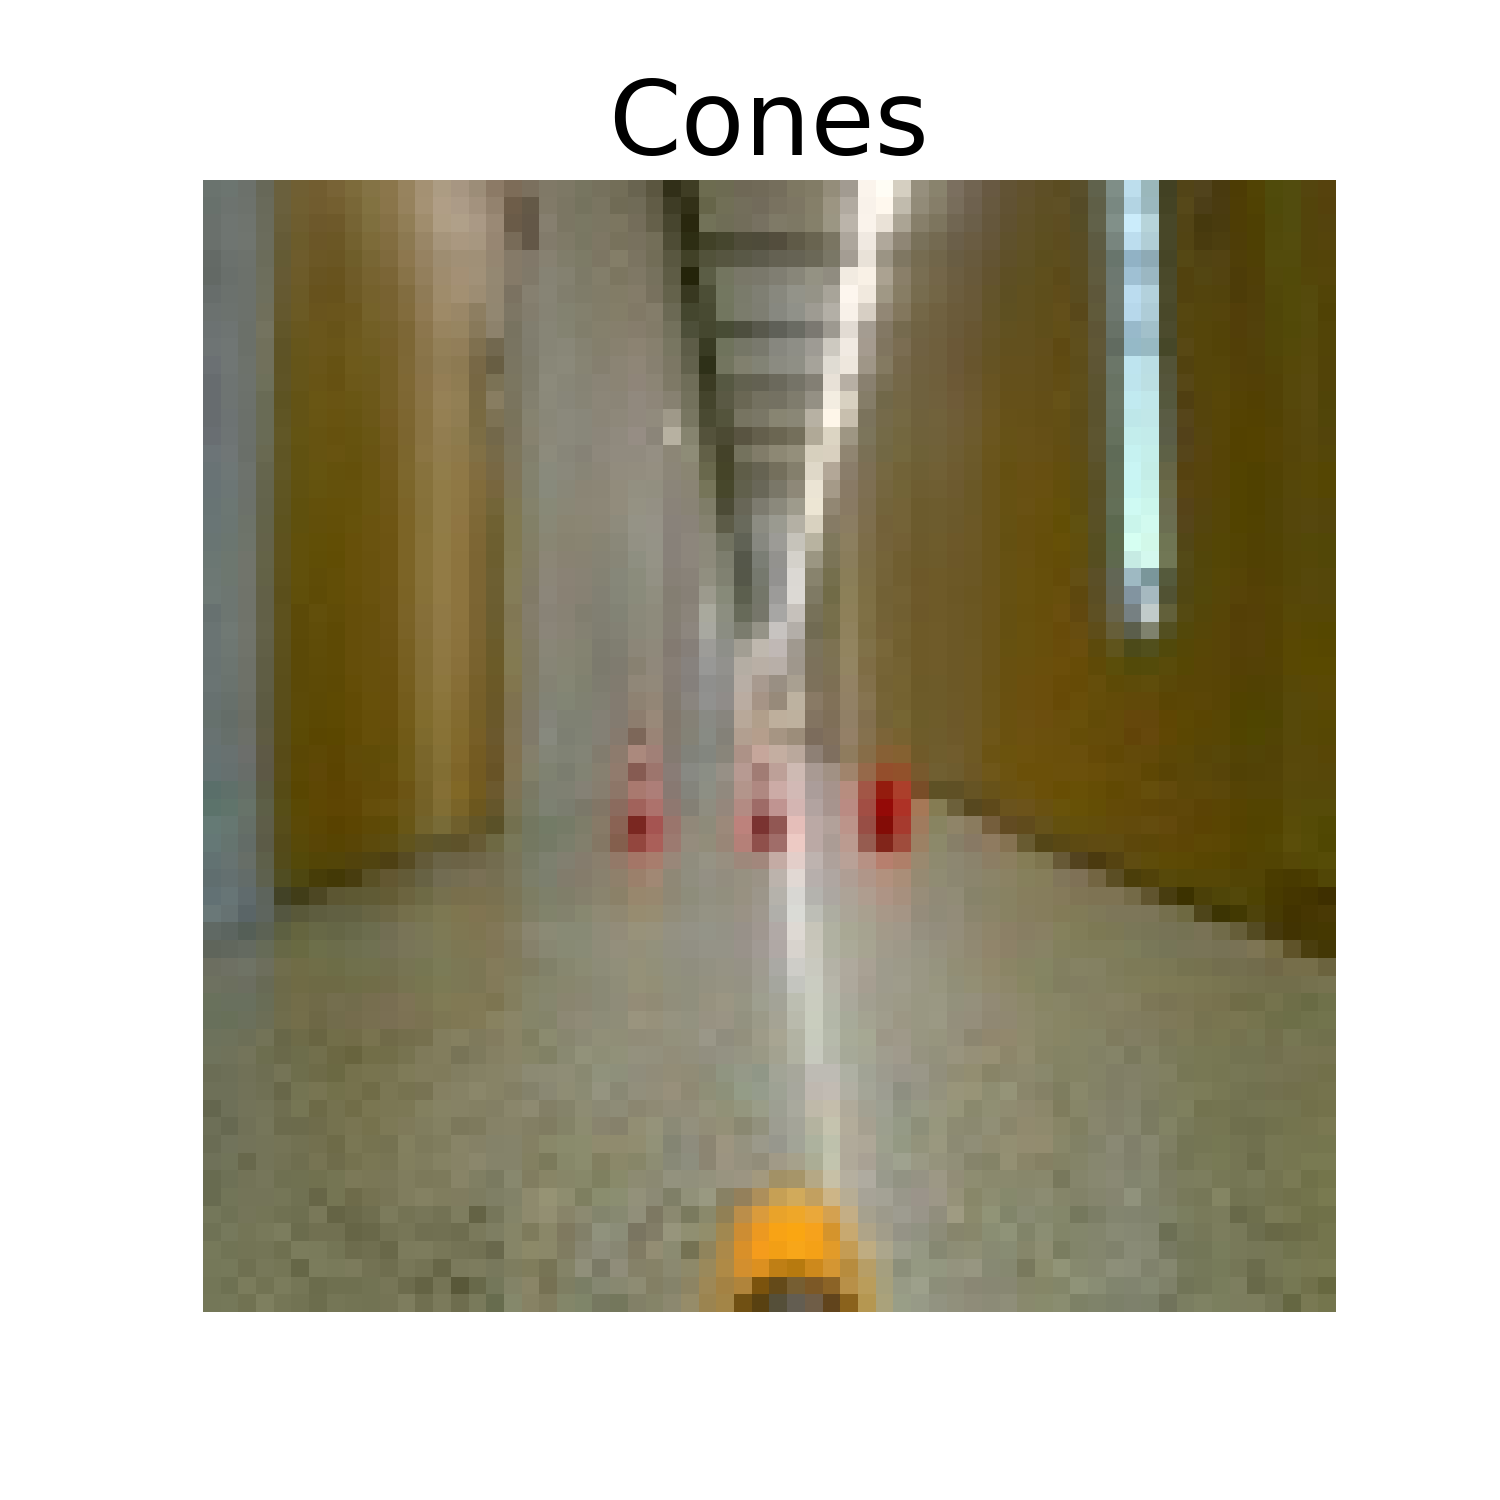
\includegraphics[width=0.29\columnwidth]{img/labels/cones.png}
        %         \label{fig:label-cones}
        %         }
        %     \subfloat[]{
        %         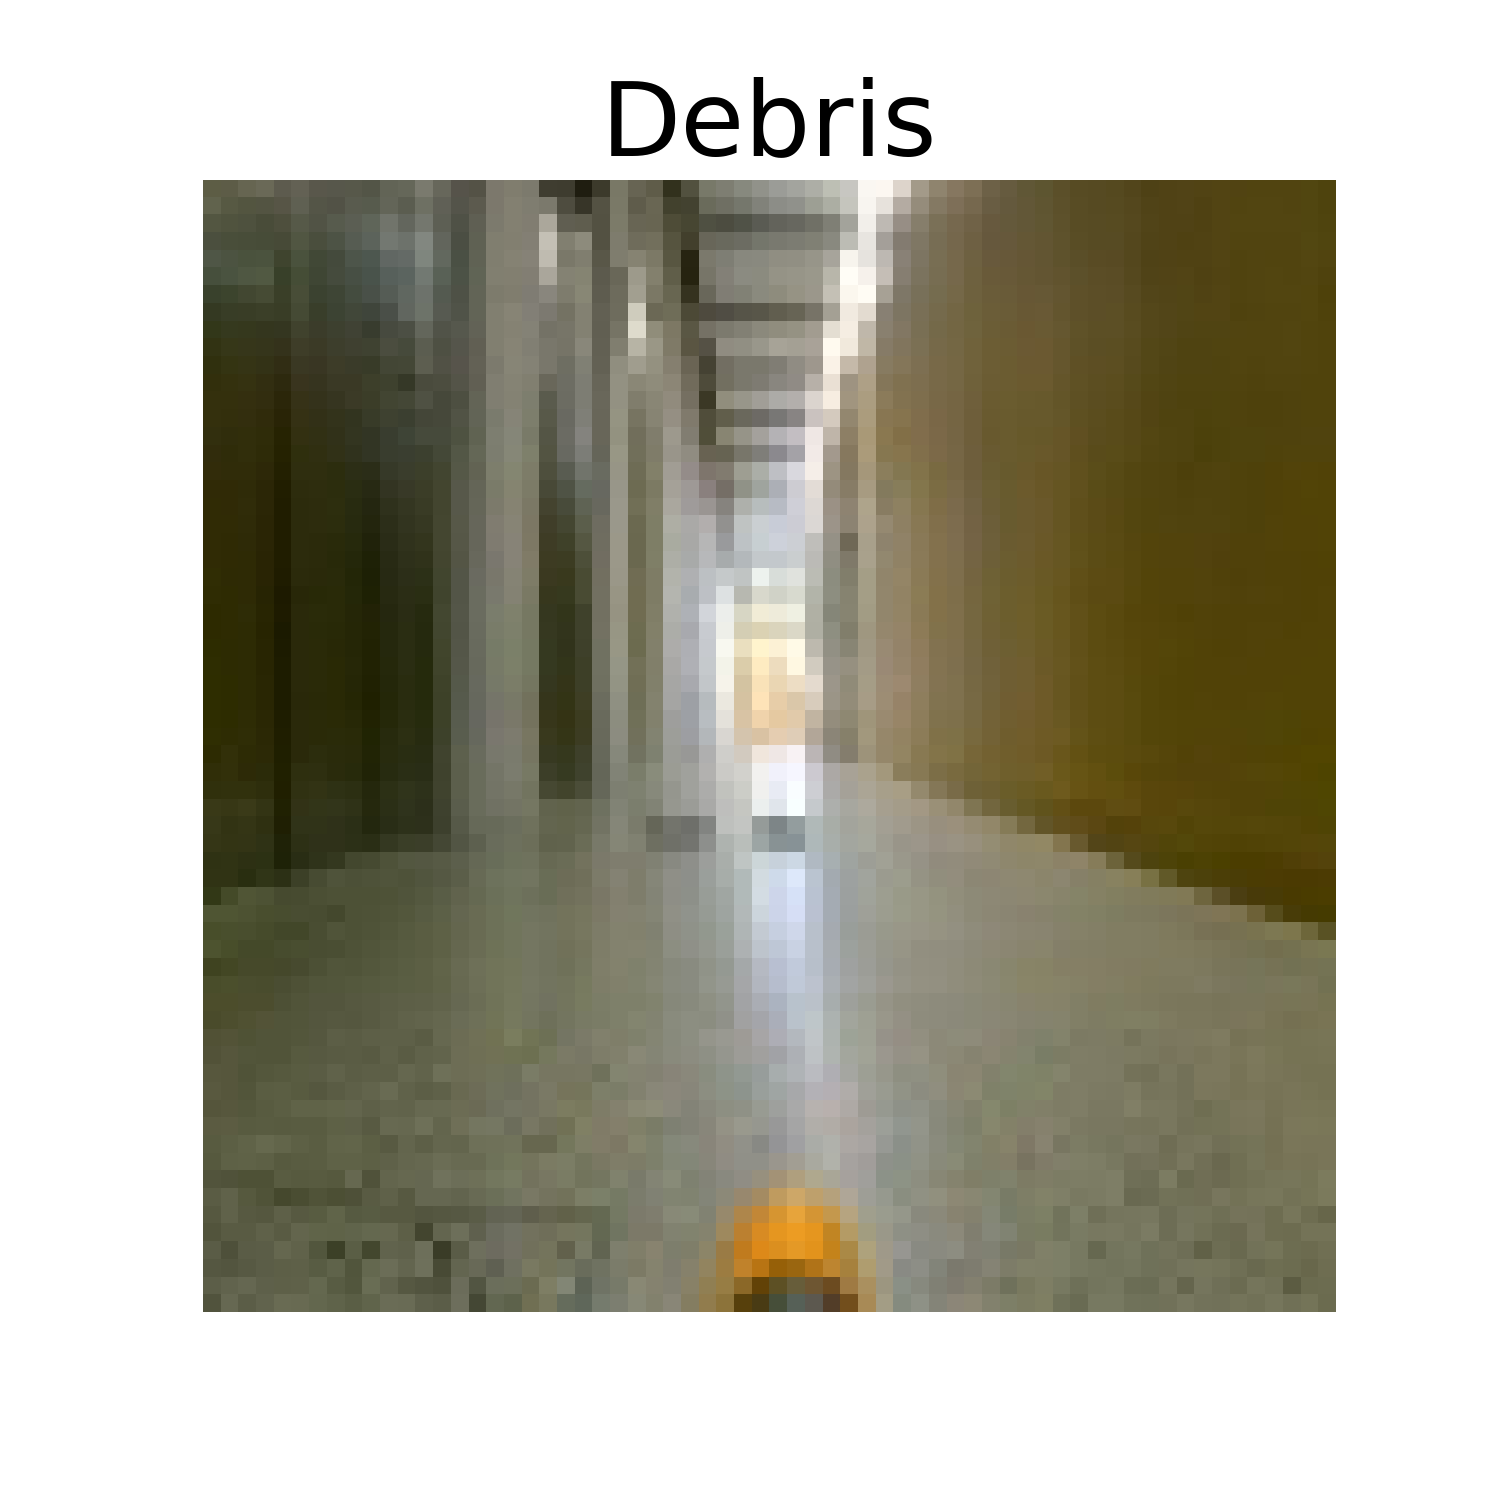
\includegraphics[width=0.29\columnwidth]{img/labels/debris.png}
        %         \label{fig:label-debris}
        %         }
        %     \subfloat[]{
        %         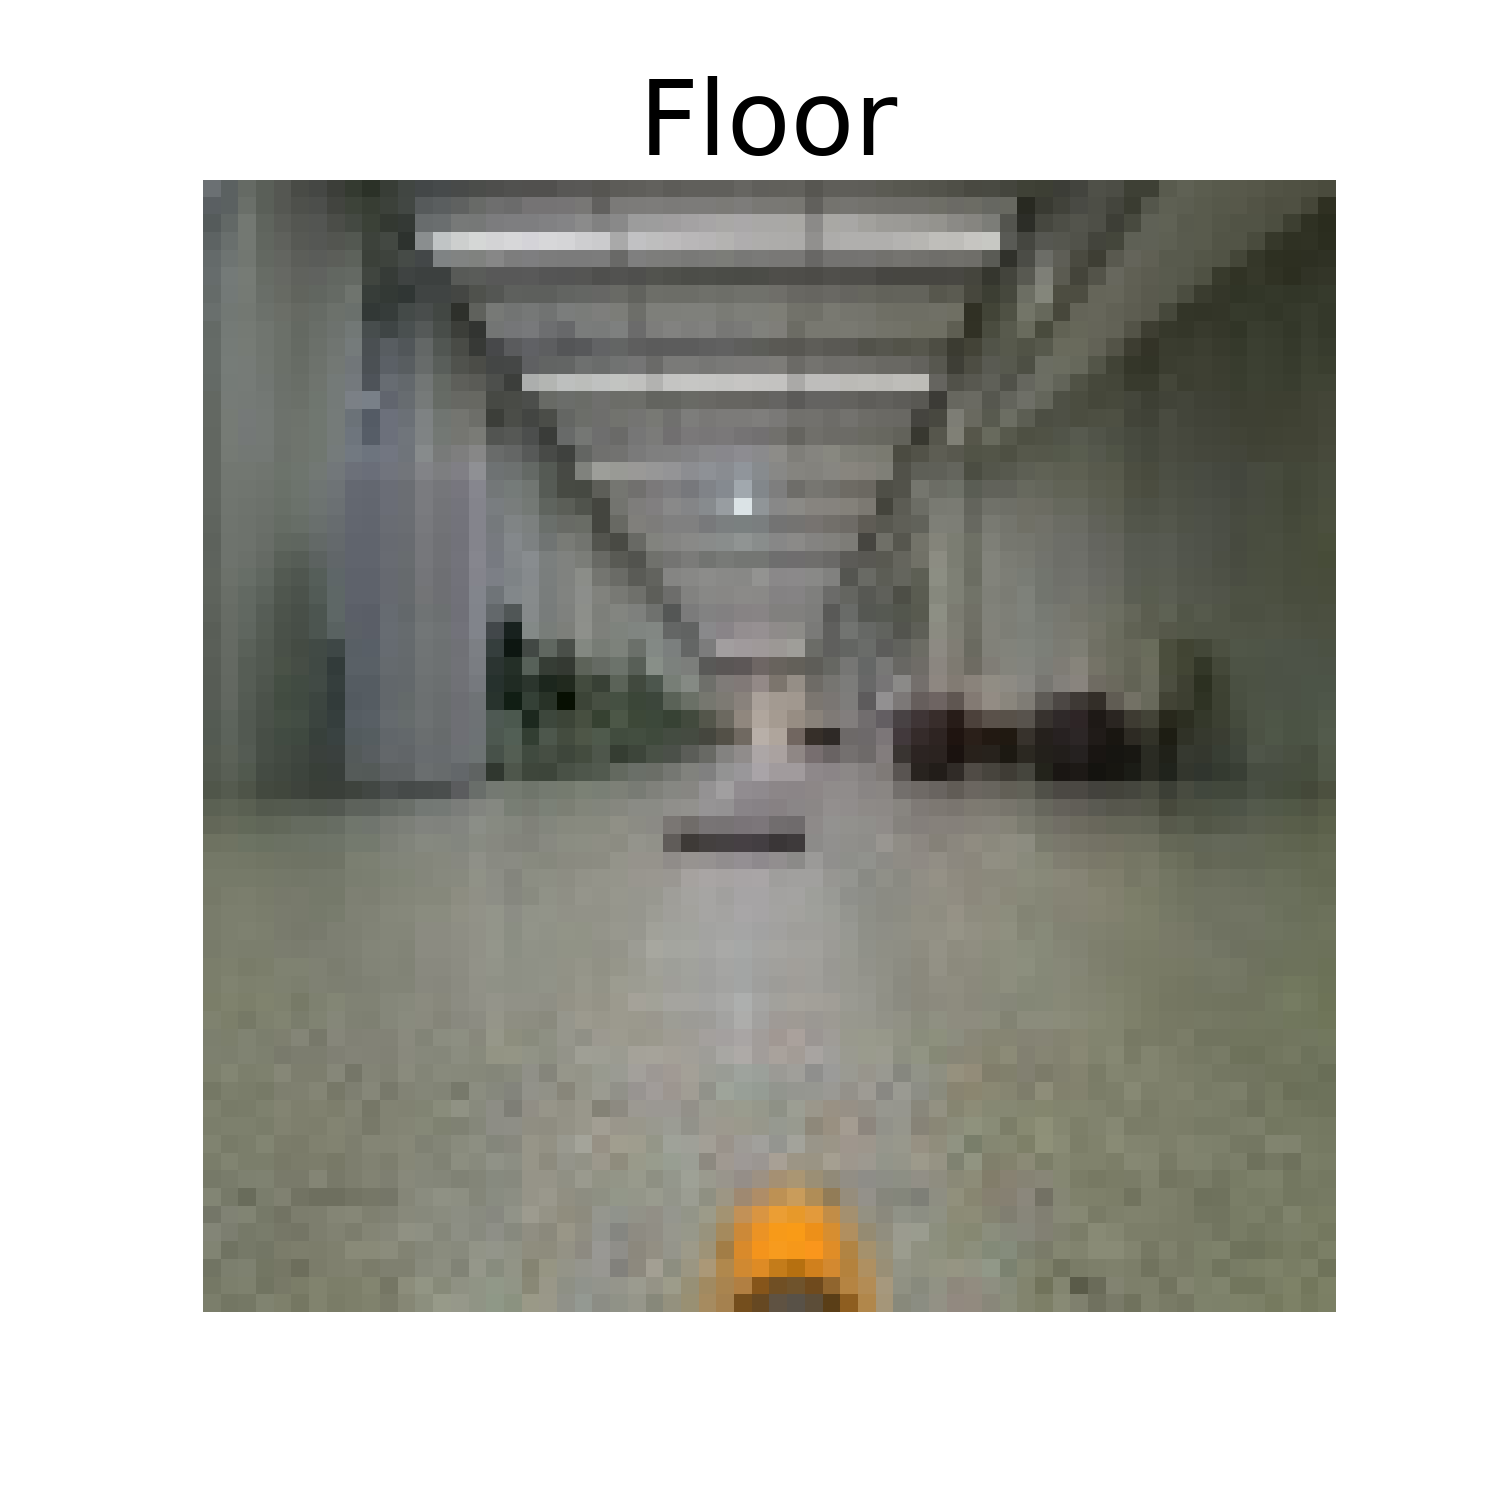
\includegraphics[width=0.29\columnwidth]{img/labels/floor.png}
        %         \label{fig:label-floor}
        %         }
        %     \\
        %     \subfloat[]{
        %         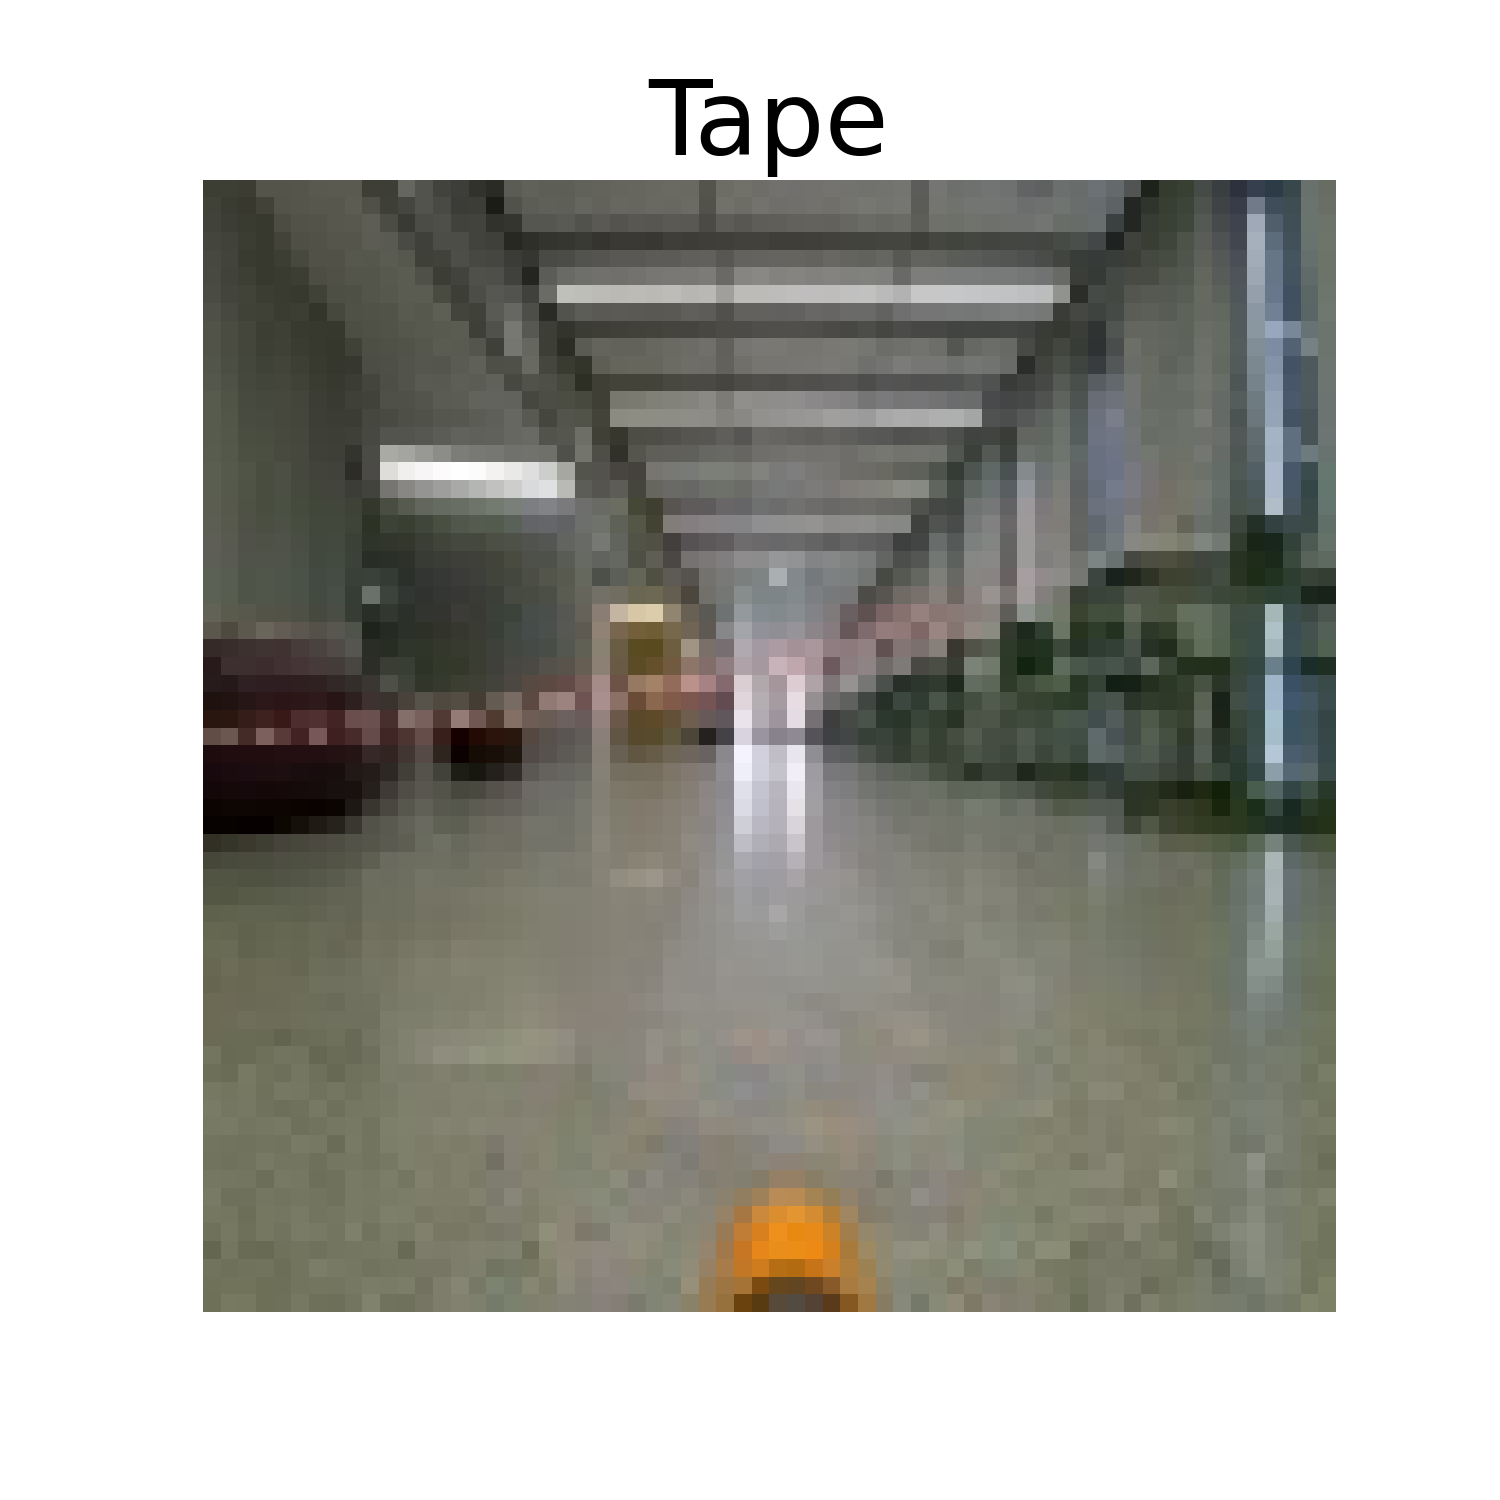
\includegraphics[width=0.29\columnwidth]{img/labels/tape.png}
        %         \label{fig:label-tape}
        %         }
        %     \subfloat[]{
        %         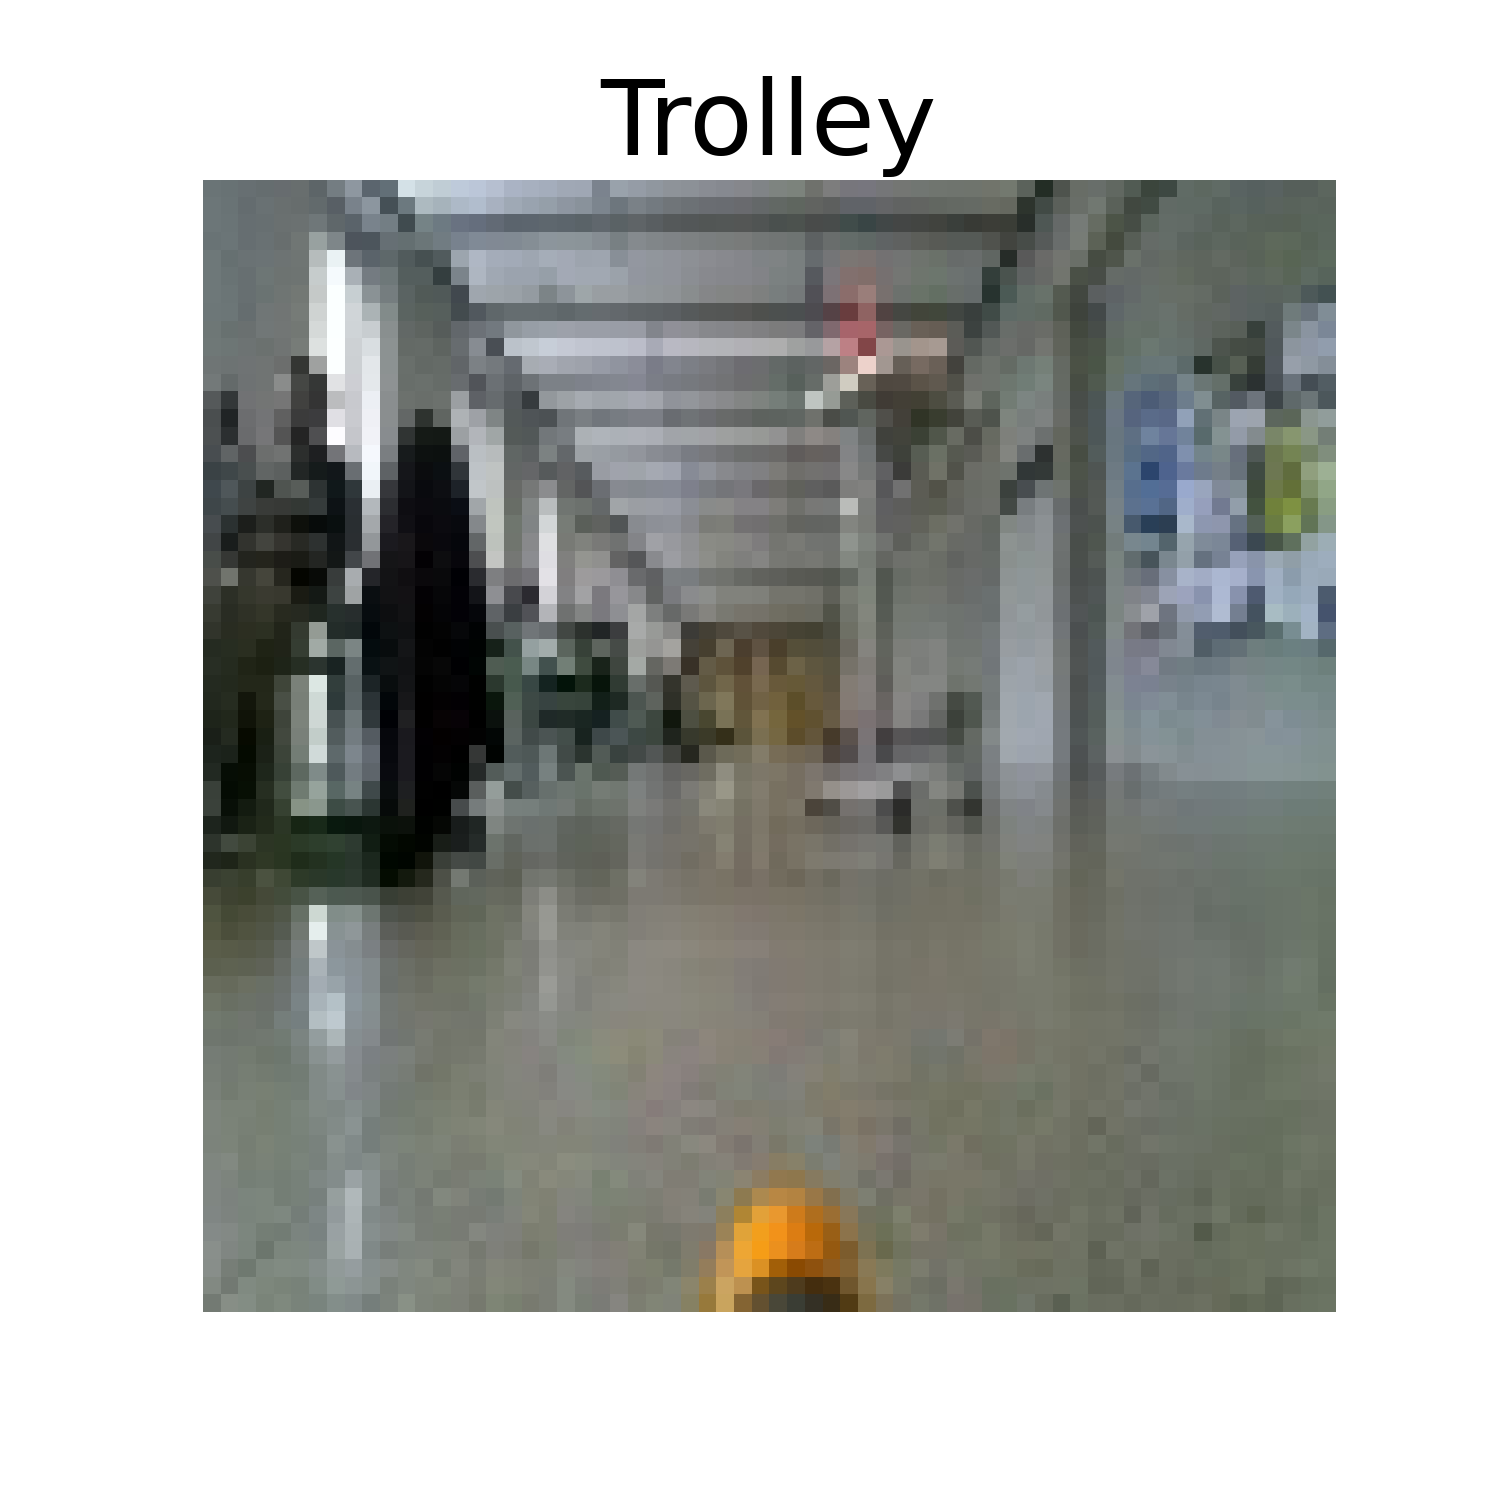
\includegraphics[width=0.29\columnwidth]{img/labels/trolley.png}
        %         \label{fig:label-trolley}
        %         }
        %     \subfloat[]{
        %         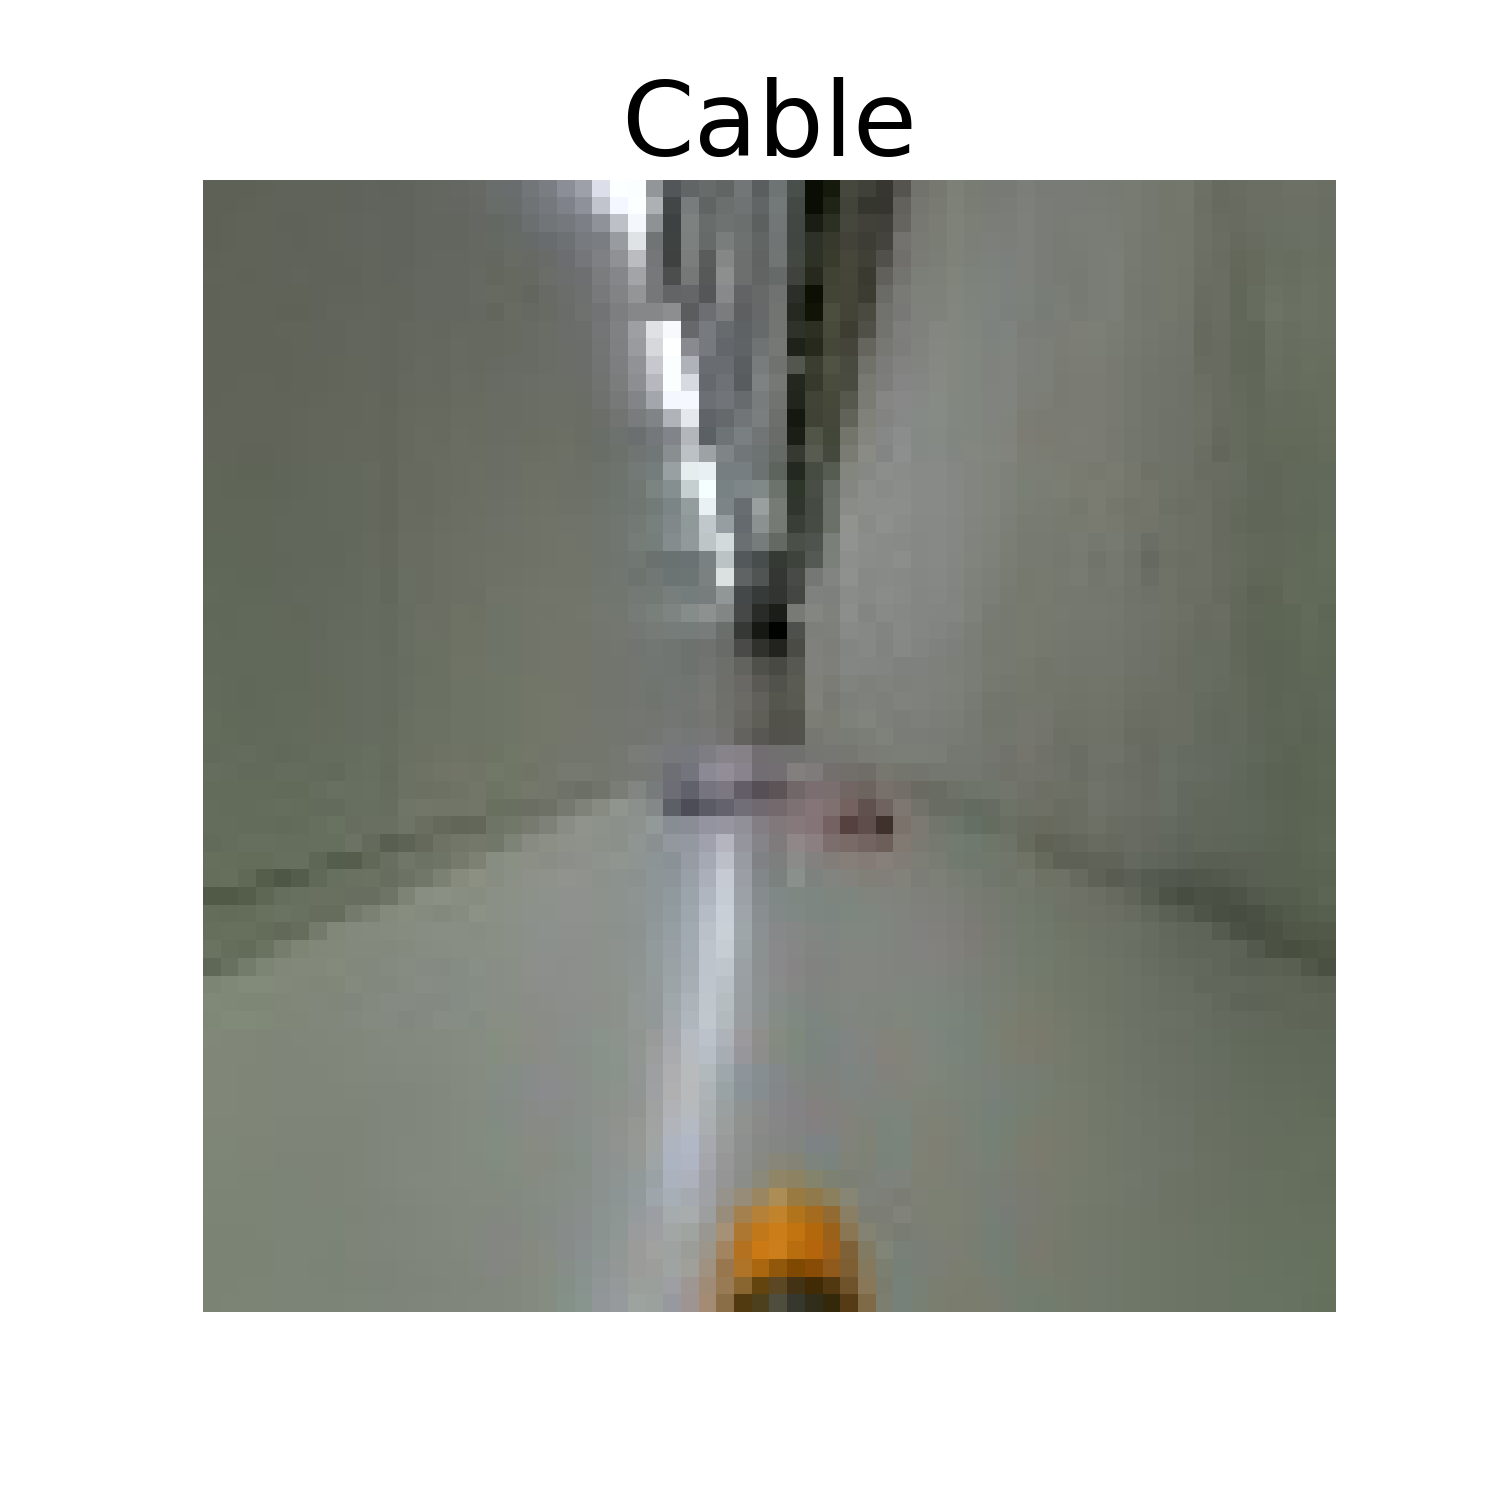
\includegraphics[width=0.29\columnwidth]{img/labels/cable.png}
        %         \label{fig:label-cable}
        %         }
        %     \\
        %     \subfloat[]{
        %         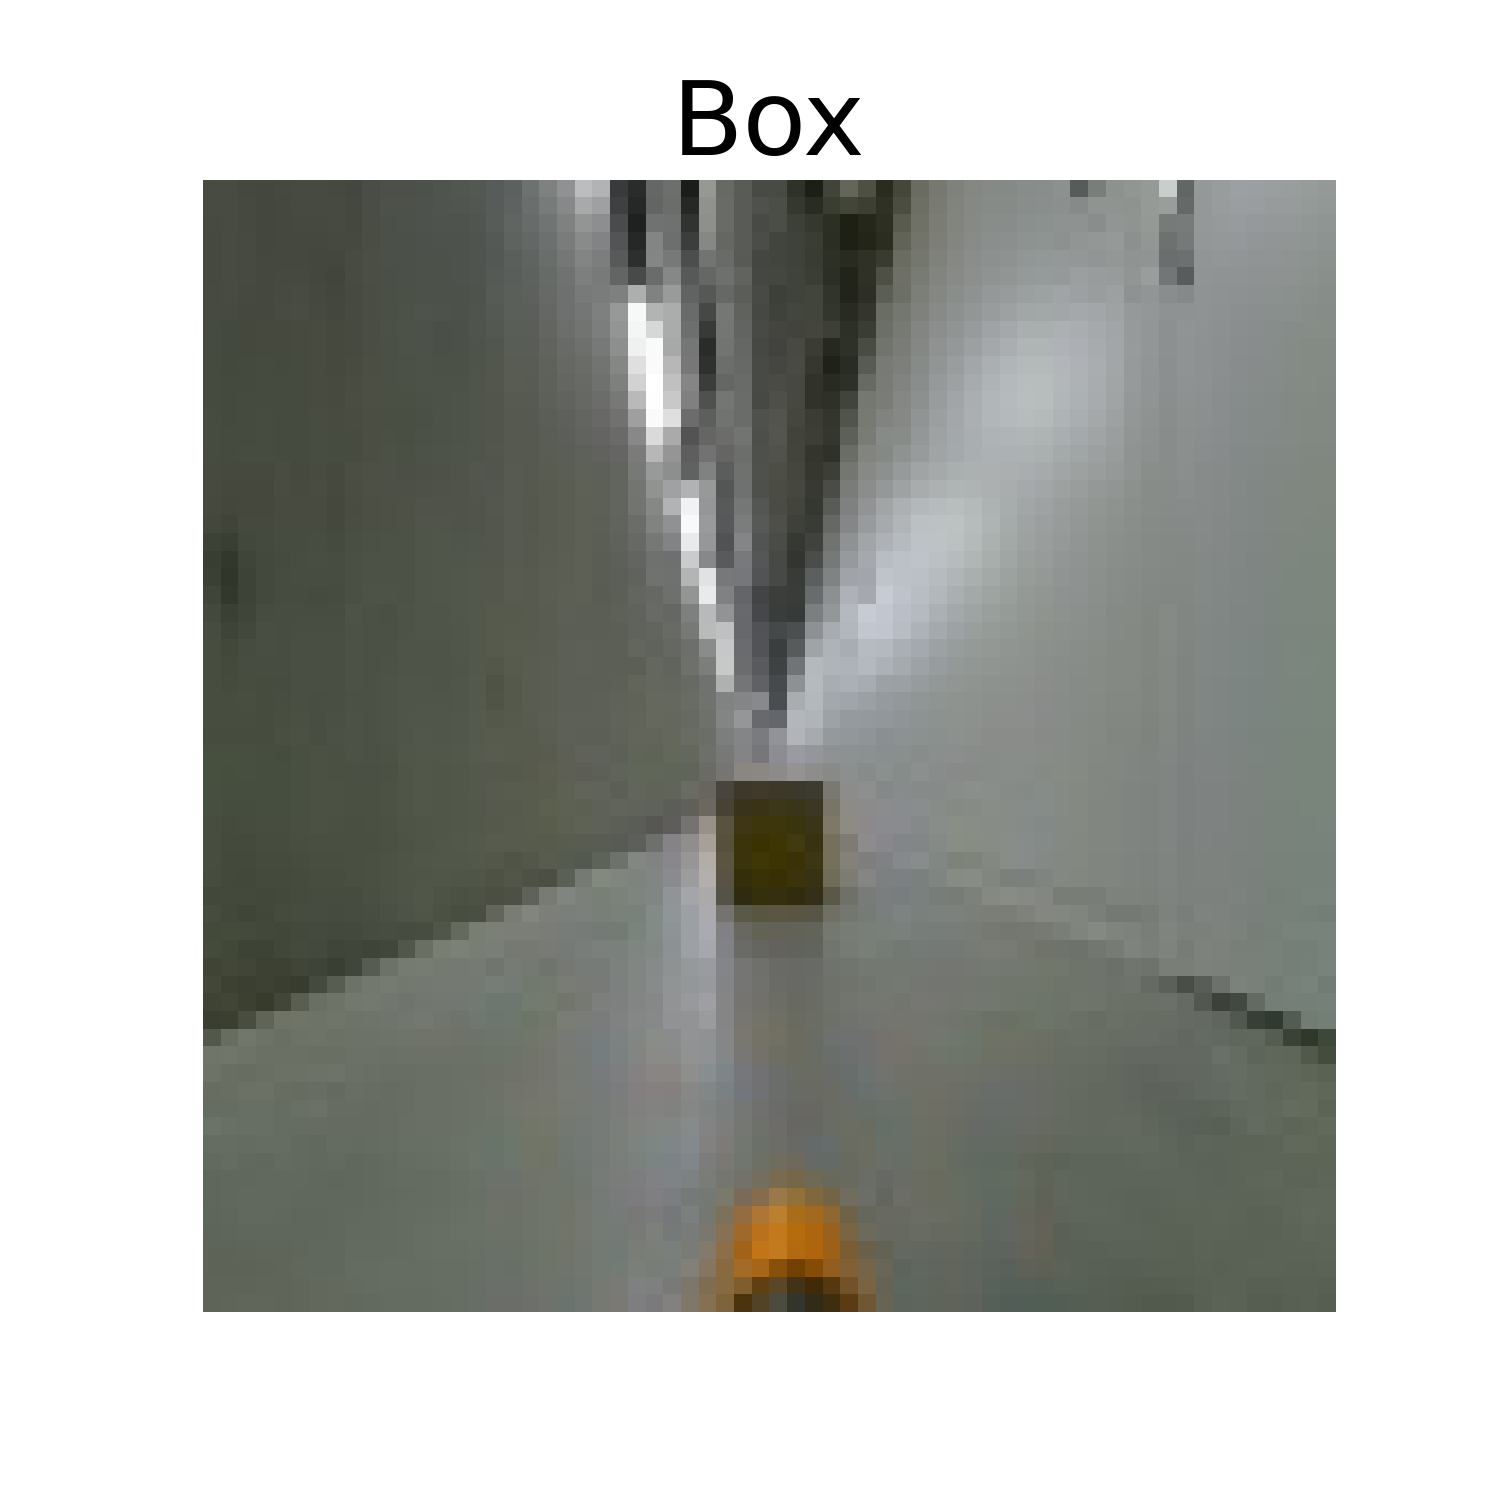
\includegraphics[width=0.29\columnwidth]{img/labels/box.png}
        %         \label{fig:label-box}
        %         }
        %     \caption{Images for each corresponding label of the short section of the dataset}
        %     \label{fig:labels-short}
        % \end{figure}

        \subsubsection*{Cones}
            The cones class (\autoref{fig:label-cones}) contains frames where the path is obstructed by cones. The cones are usually placed in front of the camera, but they can also be placed on the sides.
            \begin{figure}[H]
                \centering
                \centerline{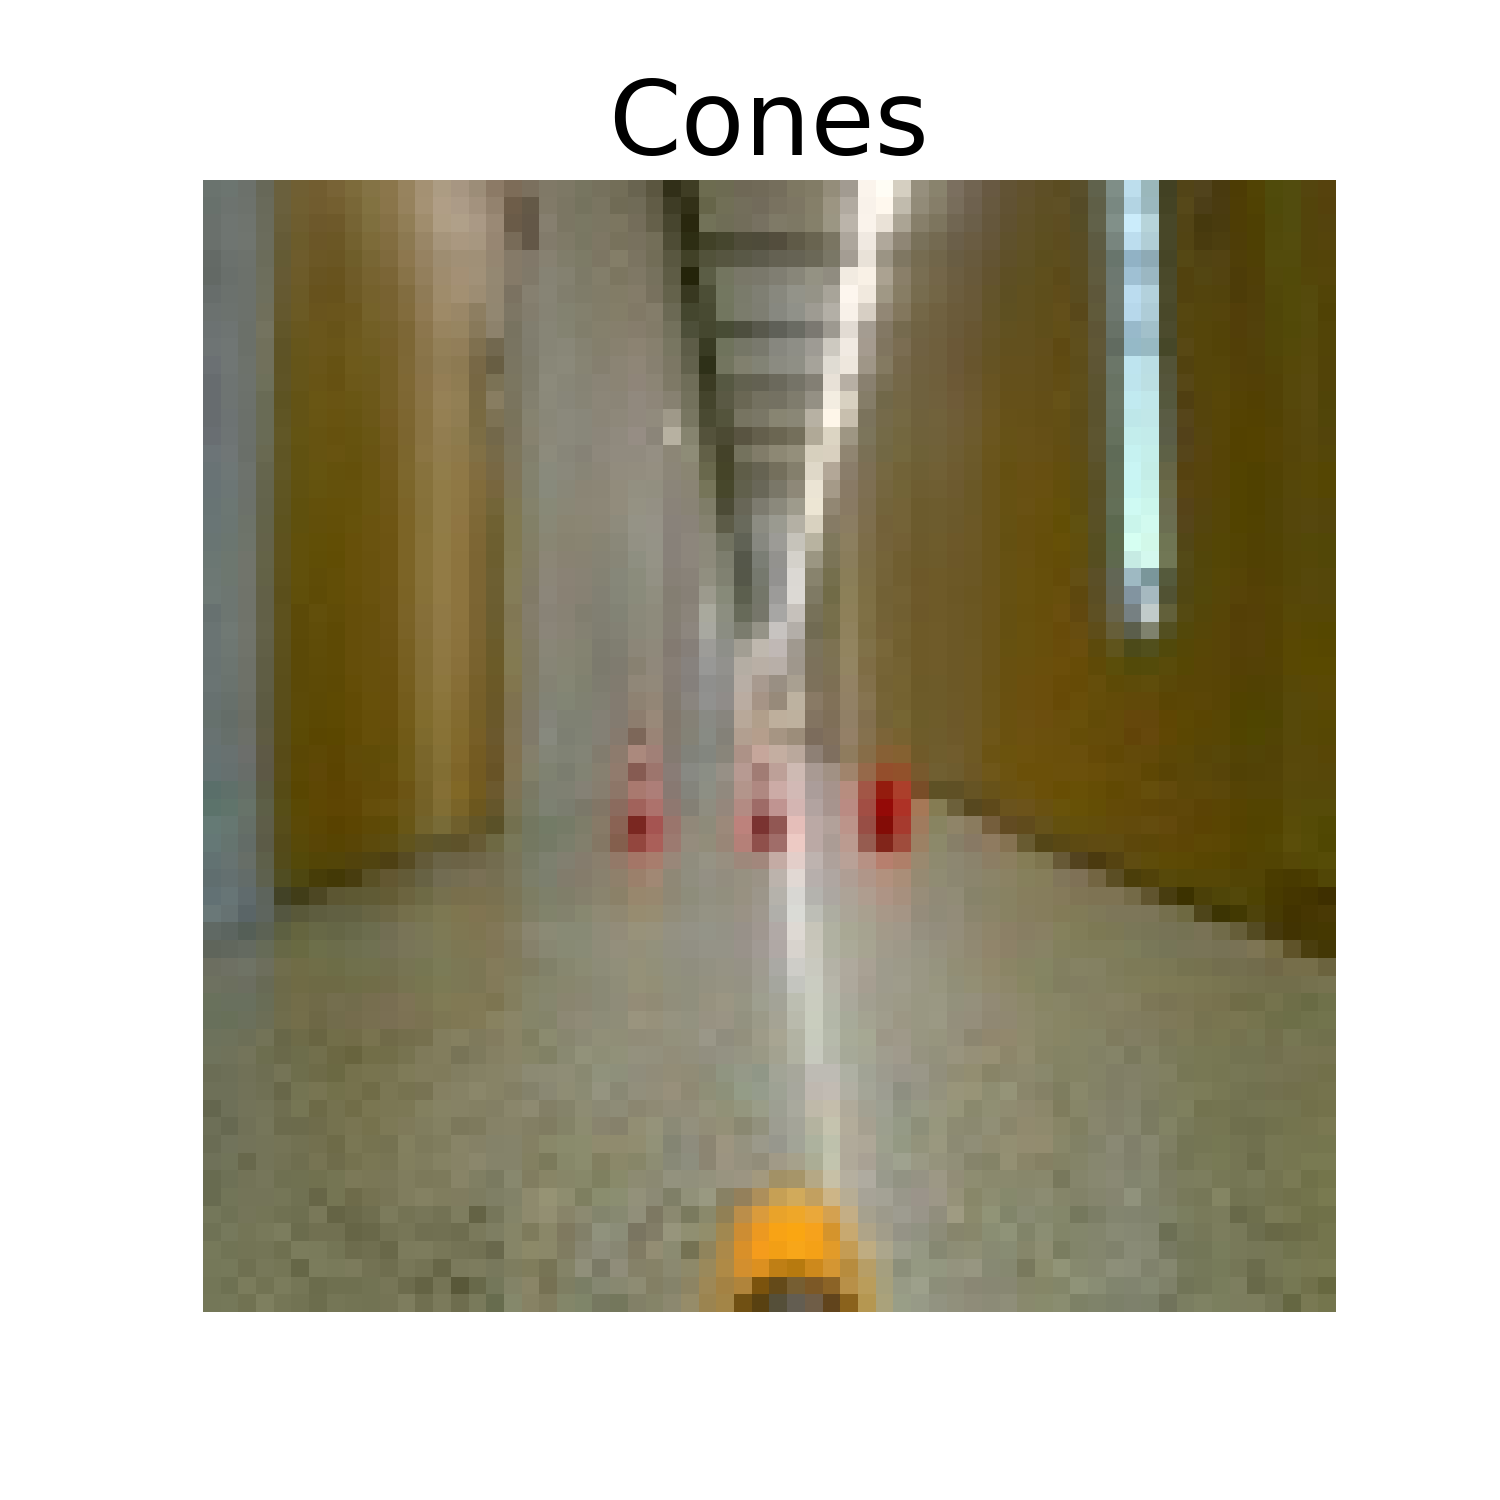
\includegraphics[width=0.75\textwidth]{img/labels/cones.png}}
                \caption{Robots\&Hazards dataset Corridors scenario, label cones}
                \label{fig:label-cones}
            \end{figure}

        \subsubsection*{Debris}
            The debris class (\autoref{fig:label-debris}) contains frames where the camera is obstructed by some kind of debris. The debris can be a piece of concrete, a piece of wood, or a piece of plastic. This anomaly is simulated by placing in front of the robot a broken concrete slab. 
            \begin{figure}[H]
                \centering
                \centerline{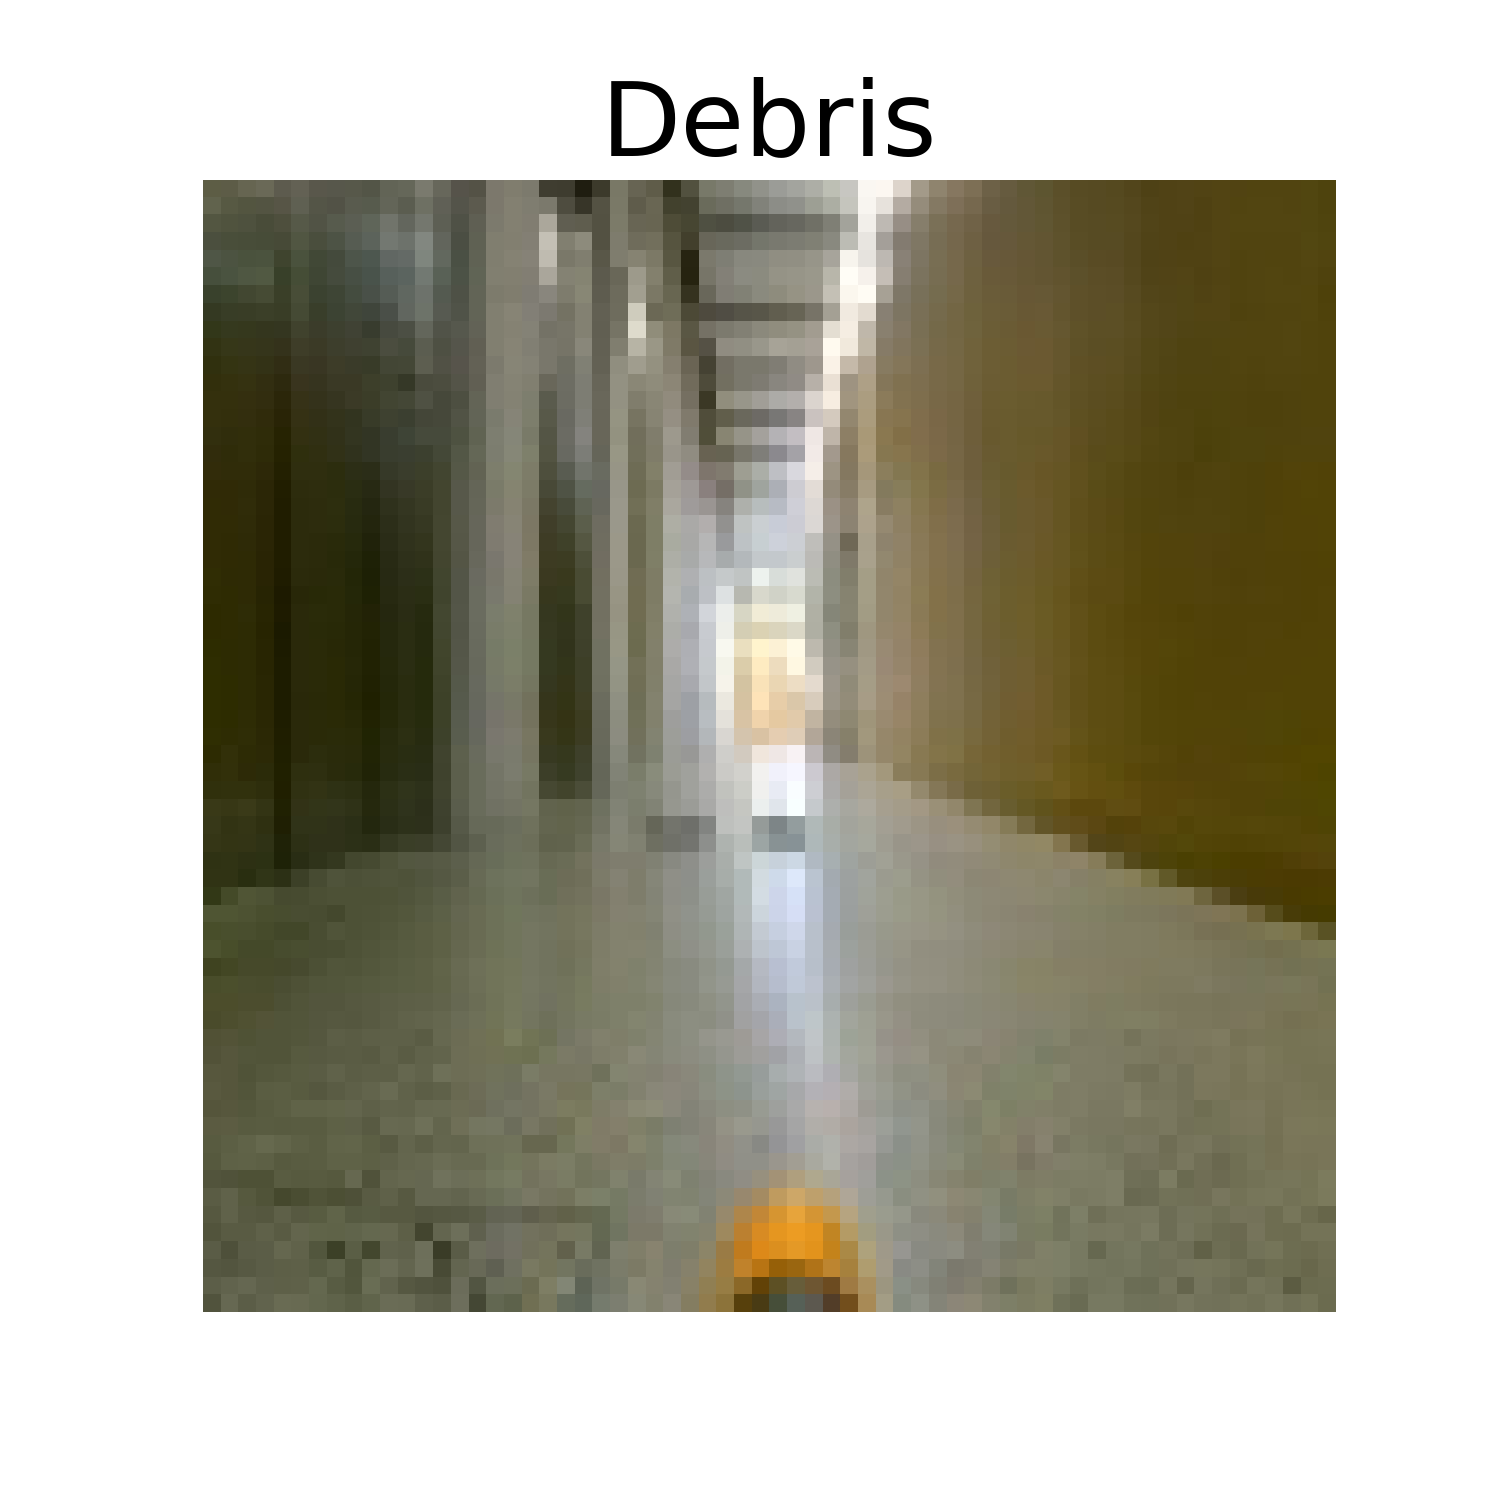
\includegraphics[width=0.75\textwidth]{img/labels/debris.png}}
                \caption{Robots\&Hazards dataset Corridors scenario, label debris}
                \label{fig:label-debris}
            \end{figure}

        \subsubsection*{Floor}
            The floor class (\autoref{fig:label-floor}) contains frames where the path is obstructed by some floor anomaly. The anomaly is simulated by placing a carpet on the floor.
            \begin{figure}[H]
                \centering
                \centerline{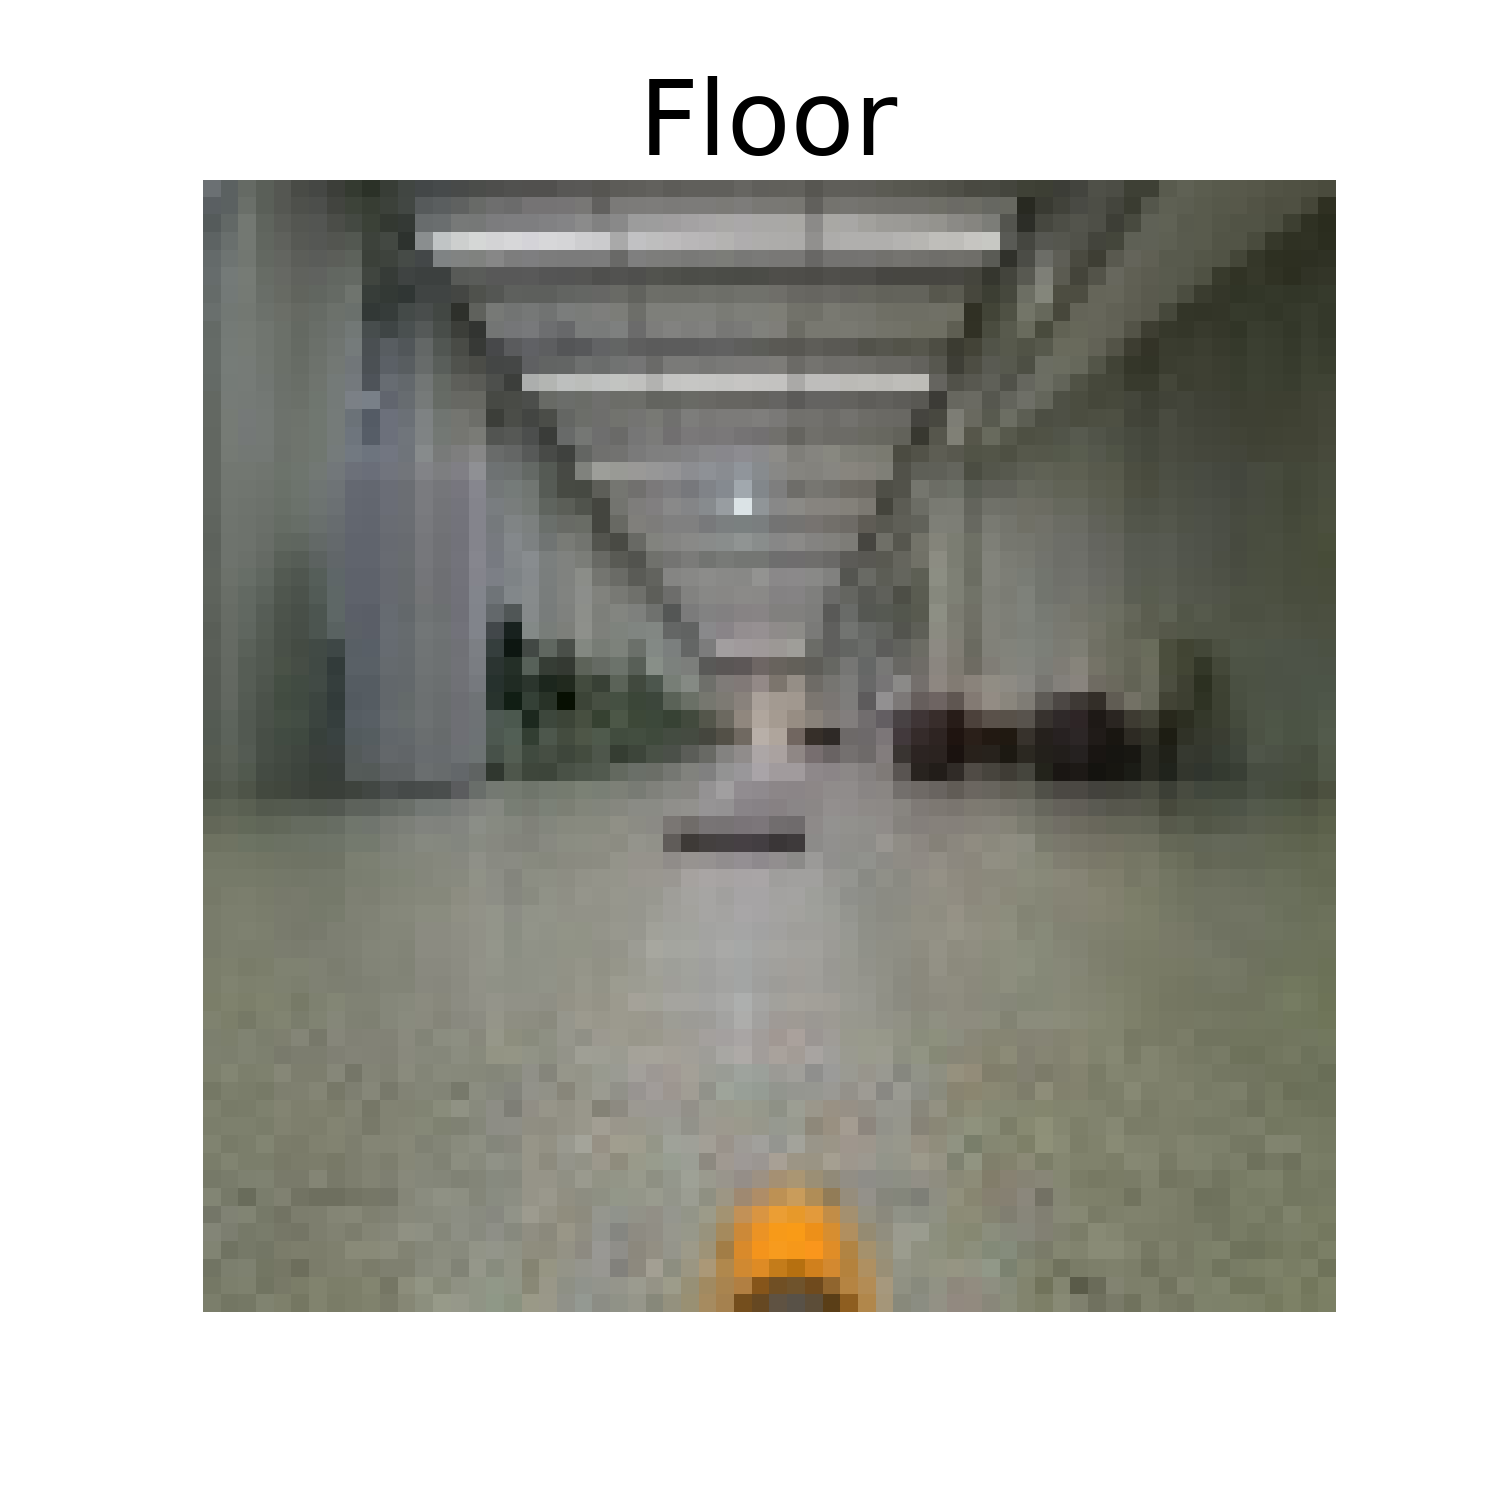
\includegraphics[width=0.75\textwidth]{img/labels/floor.png}}
                \caption{Robots\&Hazards dataset Corridors scenario, label floor}
                \label{fig:label-floor}
            \end{figure}
        
        \subsubsection*{Tape}
            The tape class (\autoref{fig:label-tape}) contains frames where the path is obstructed by some tape placed at random heights, even higher than the robot's height.
            \begin{figure}[H]
                \centering
                \centerline{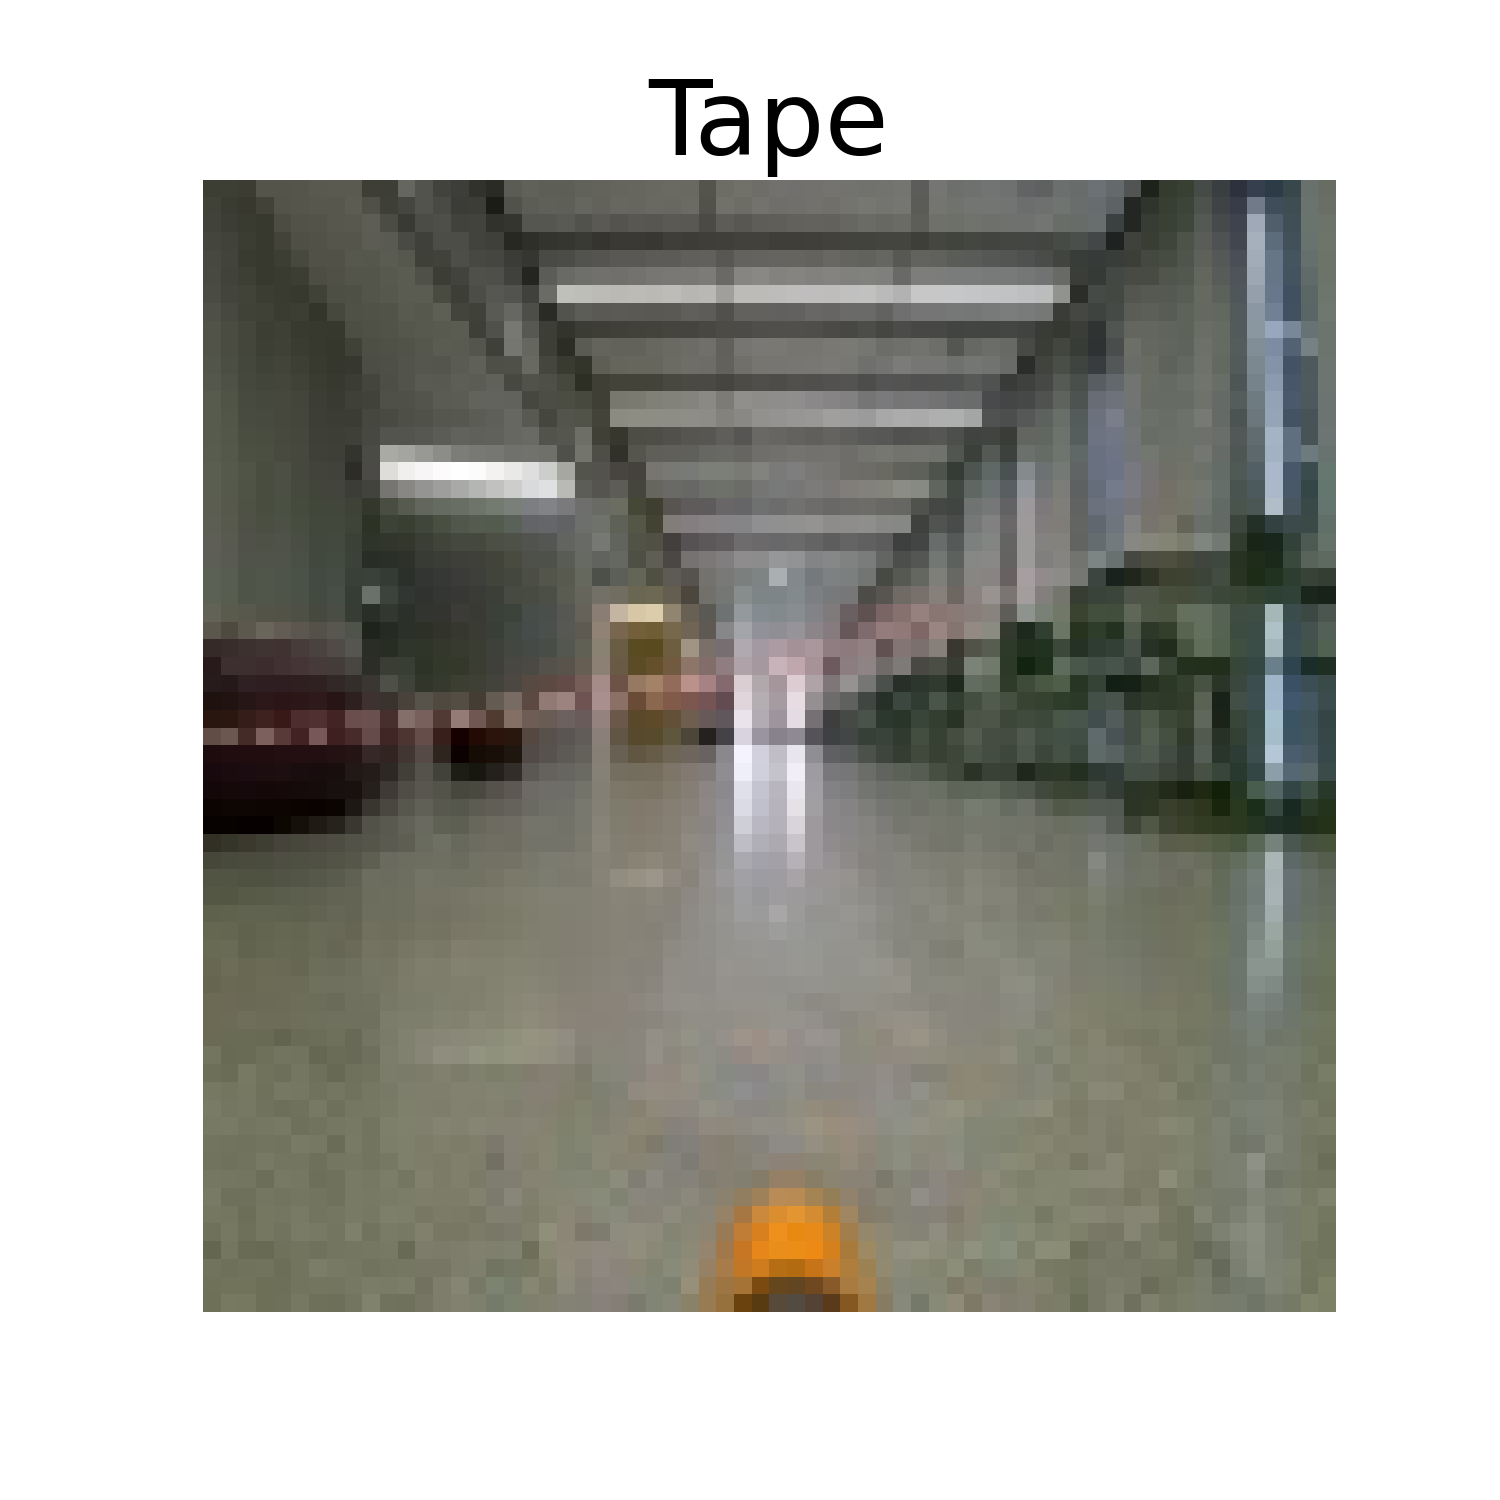
\includegraphics[width=0.75\textwidth]{img/labels/tape.png}}
                \caption{Robots\&Hazards dataset Corridors scenario, label tape}
                \label{fig:label-tape}
            \end{figure} 

        \subsubsection*{Trolley}
            The trolley class (\autoref{fig:label-trolley}) contains frames where the path is obstructed by a trolley. The trolley can be a small or large.
            \begin{figure}[H]
                \centering
                \centerline{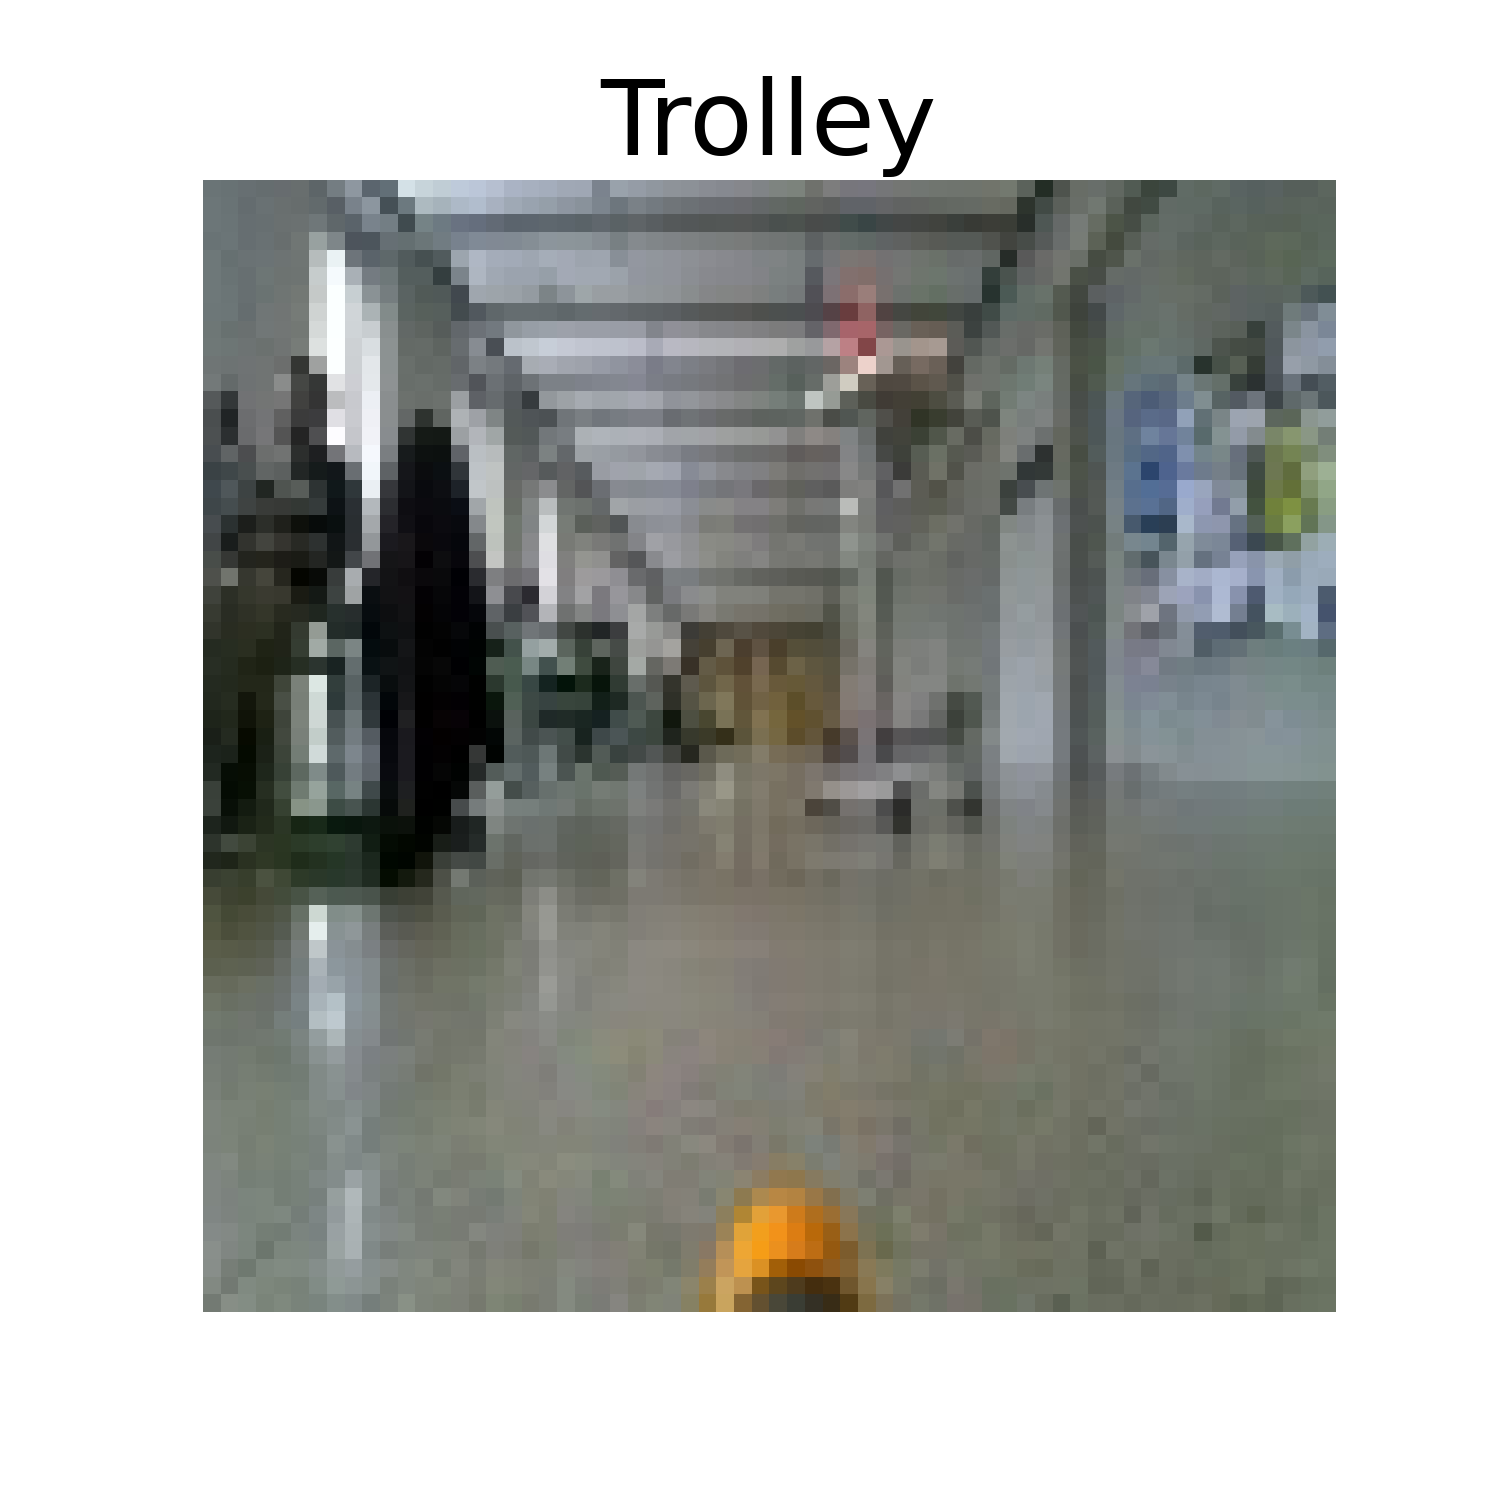
\includegraphics[width=0.75\textwidth]{img/labels/trolley.png}}
                \caption{Robots\&Hazards dataset Corridors scenario, label trolley}
                \label{fig:an-trolley}
            \end{figure}

        \subsubsection*{Cable}
            The cable class (\autoref{fig:label-cable}) contains frames where the path is obstructed by a cable. The cable can be a power cable, a network cable, or a USB cable.
            \begin{figure}[H]
                \centering
                \centerline{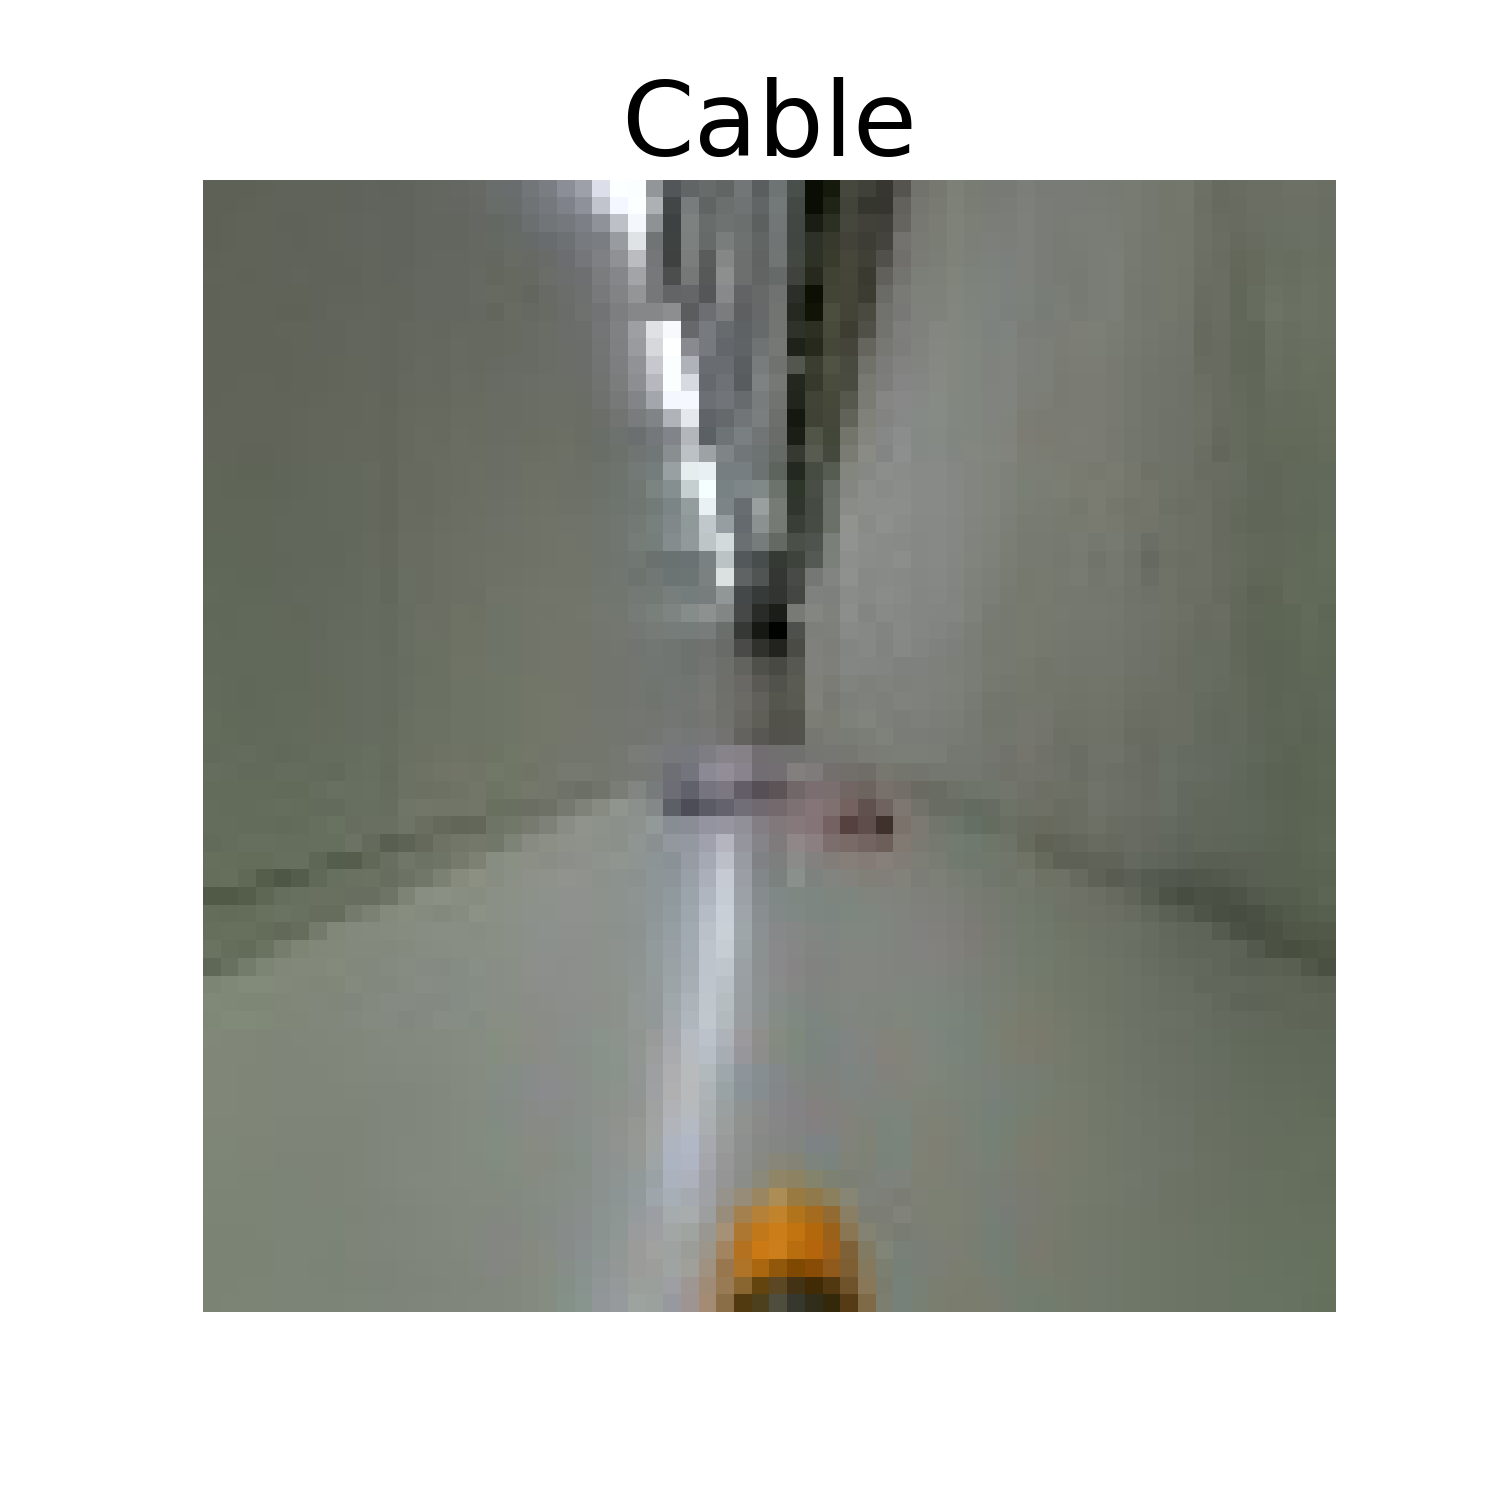
\includegraphics[width=0.75\textwidth]{img/labels/cable.png}}
                \caption{Robots\&Hazards dataset Corridors scenario, label cable}
                \label{fig:an-cable}
            \end{figure}

        \subsubsection*{Box}
            The box class (\autoref{fig:label-box}) contains frames where the camera is obstructed by a box. The box can be of any size.
            \begin{figure}[H]
                \centering
                \centerline{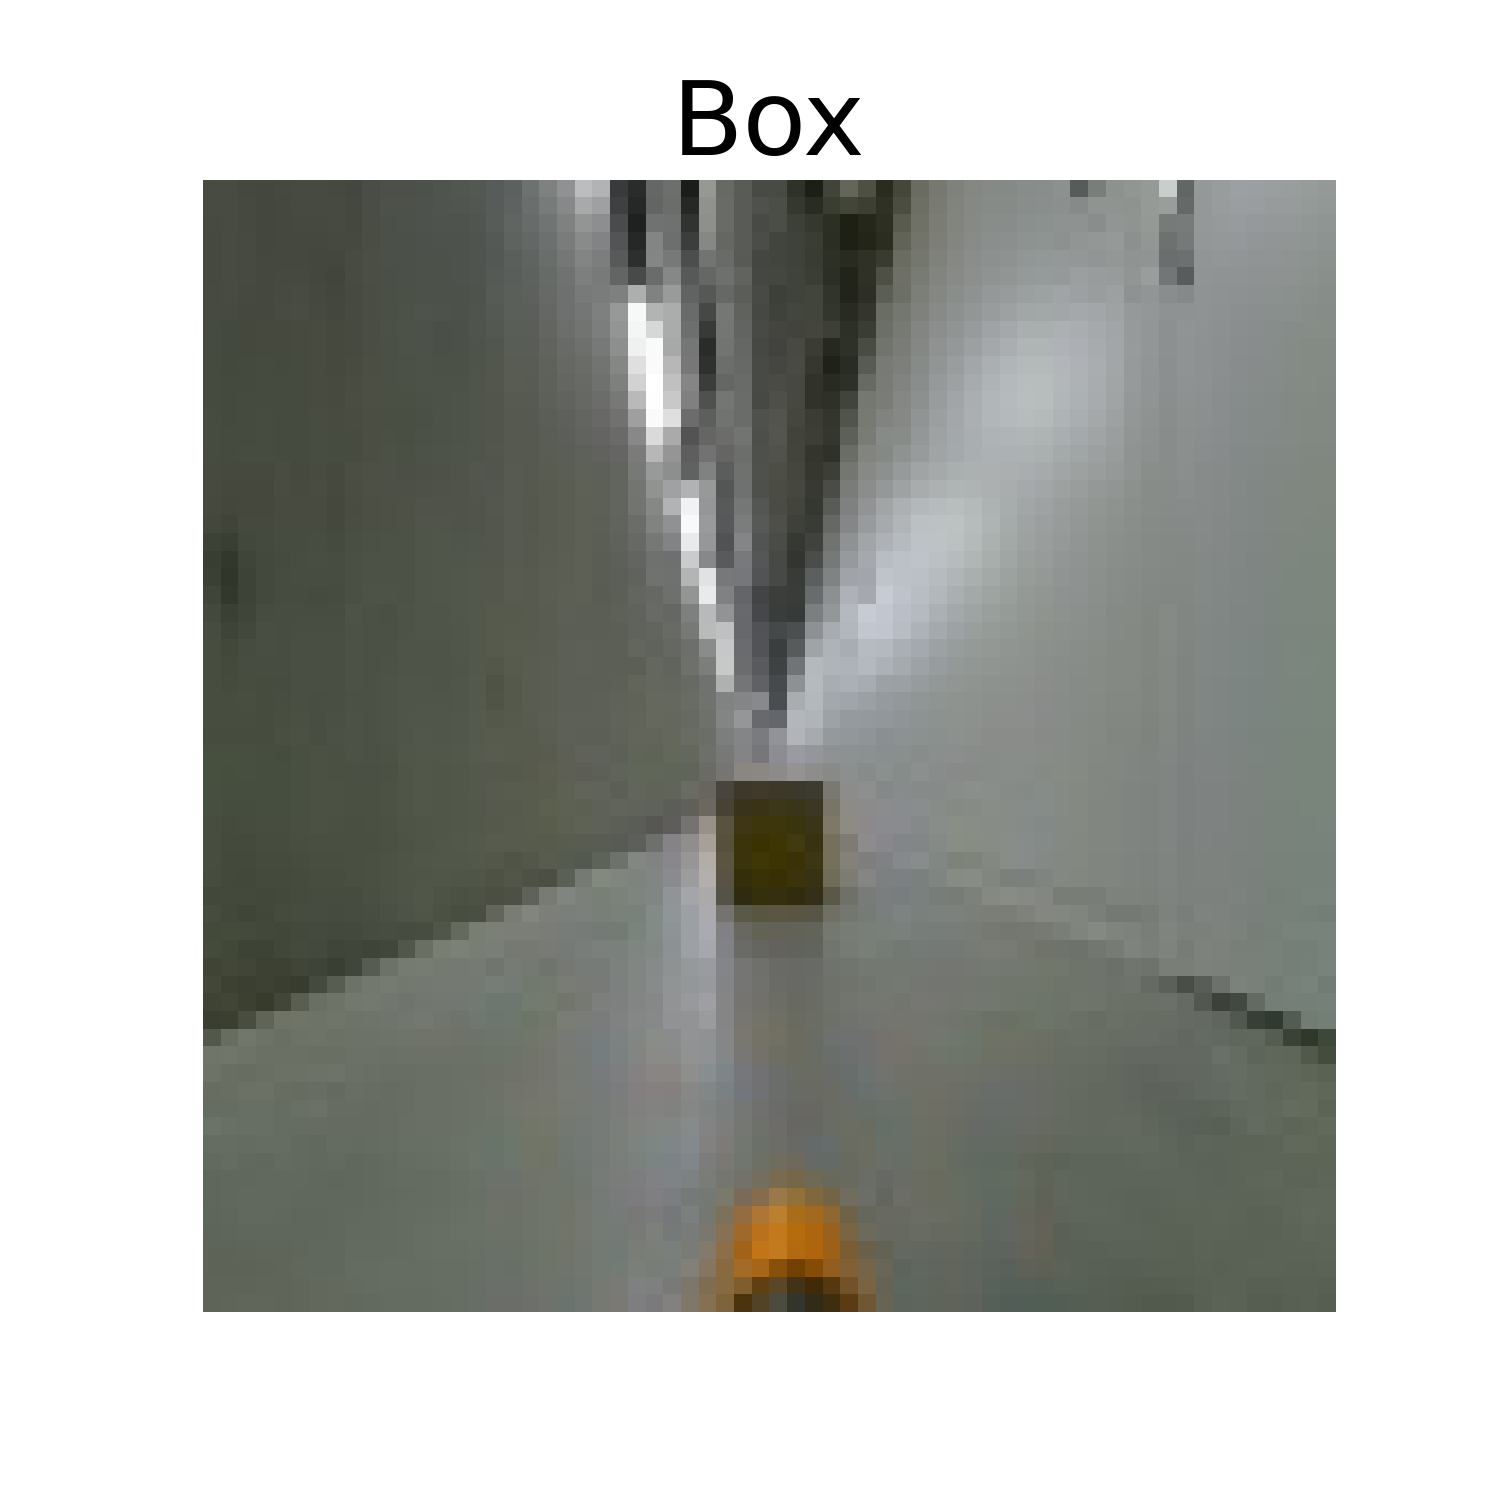
\includegraphics[width=0.75\textwidth]{img/labels/box.png}}
                \caption{Robots\&Hazards dataset Corridors scenario, label box}
                \label{fig:an-box}
            \end{figure}
    